
% ==========================================
% CHAPITRE 3
% ==========================================
\newpage
\chapter{Étude et Réalisation du Premier Sprint}
\vspace{2.5cm}

\noindent \textbf{\Large Plan}
\vspace{0.8cm}
\begin{enumerate}[label=\textbf{\arabic*}, leftmargin=1.5cm, labelsep=0.8cm]
    \item[] \hspace*{-1.5cm}\textbf{Introduction} \dotfill \pageref{sec:s1-intro}
    \item \textbf{User Stories du premier sprint} \dotfill \pageref{sec:s1-userstories}
    \item \textbf{Backlog du premier Sprint} \dotfill \pageref{sec:s1-backlog}
    \item \textbf{Spécification fonctionnelle} \dotfill \pageref{sec:s1-specification}
    \item \textbf{Conception du premier Sprint} \dotfill \pageref{sec:s1-conception}
    \item \textbf{Etude et réalisation} \dotfill \pageref{sec:s1-realisation}
    \item \textbf{Tests et Validation} \dotfill \pageref{sec:s1-tests}
    \item \textbf{Rituels Agiles } \dotfill \pageref{sec:s1-rituels}
    \item[] \hspace*{-1.5cm}\textbf{Conclusion} \dotfill \pageref{sec:s1-conclusion}
\end{enumerate}
\vfill
\newpage

\section*{Introduction}
\label{sec:s1-intro}

\addcontentsline{toc}{section}{Introduction}
Ce chapitre détaille les travaux réalisés lors du premier sprint de développement de
  PaieZone~RH. L'objectif de ce sprint était de construire le socle technique et fonctionnel
  de la plateforme, couvrant six domaines prioritaires~: le mécanisme d'authentification
  multi-rôles avec redirection contextuelle, le provisionnement automatique des espaces
  société (Tenant Provisioning), la gestion des abonnements SaaS, l'administration des
  comptes utilisateurs avec flux d'invitation par e-mail, le journal d'audit automatique par
  interception AOP, et la structuration organisationnelle (départements et postes).

  La démarche adoptée pour ce sprint suit le cycle Scrum~: planification via les User Stories,
  spécification par diagrammes de cas d'utilisation UML, conception technique par diagrammes
  de classes et de séquences, réalisation des interfaces Angular, puis validation par un plan
  de tests multiniveaux et clôture agile (Sprint Review et Rétrospective).
% ============================================================
\section{User Stories du premier sprint}
\label{sec:s1-userstories}
% ============================================================

Conformément aux méthodologies agiles, l'équipe Scrum a initié ce sprint par une réunion de planification dédiée à la formulation de l'objectif du sprint. Cet objectif, exprimé en termes métier, vise à garantir une compréhension unifiée et partagée par toutes les parties prenantes, internes comme externes à l'équipe de développement.

La question fondamentale à laquelle ce sprint répond est « Quelle valeur métier ce sprint apporte-t-il ? ». Pour ce premier incrément, l'objectif était de concrétiser les six éléments suivants du backlog, jugés prioritaires pour établir les fondations du système :

\begin{itemize}[label=\textbullet, leftmargin=0.6cm]
    \item Authentification Multi-Rôles
    \item Gestion des Entreprises
    \item Gestion des Abonnements SaaS
    \item Gestion des Utilisateurs
    \item Journal d'Audit et Traçabilité
    \item Gestion de la Structure Organisationnelle
\end{itemize}
Les besoins fonctionnels du premier sprint ont été formalisés sous forme de User Stories. 
L'intégralité de ces User Stories, incluant leurs identifiants, critères d'acceptation et 
niveaux de priorité, est détaillée dans le Tableau~\ref{tab:sprint1-us}.

\renewcommand{\arraystretch}{1.4}
\begin{small}
\begin{longtable}{|p{1.2cm}|p{9.5cm}|p{2.3cm}|}

\hline
\rowcolor[gray]{0.9}
\textbf{ID} & \textbf{User Story} & \textbf{Priorité} \\
\hline
\endfirsthead

\hline
\rowcolor[gray]{0.9}
\textbf{ID} & \textbf{User Story} & \textbf{Priorité} \\
\hline
\endhead

\hline
\endfoot
\endfoot

1.1 & En tant qu'utilisateur, je veux m'authentifier afin d'accéder au système. & Critique \\ \hline
1.2 & En tant qu'Admin, je veux m'inscrire en fournissant mes informations et celles de ma société, 
afin de créer mon espace de gestion isolé et d'en devenir le responsable. & Critique \\ \hline
2.1 & En tant qu'Admin, je veux modifier une entreprise, afin de mettre à jour ses informations 
légales. & Haute \\ \hline
2.2 & En tant qu'Admin, je veux désactiver une entreprise, afin de suspendre l'accès de l'ensemble 
de ses utilisateurs. & Haute \\ \hline
2.3 & En tant que Super Admin, je veux affecter un abonnement, afin de définir les droits et quotas 
d'une entreprise cliente. & Critique \\ \hline
2.4 & En tant que Super Admin, je veux modifier un abonnement, afin de changer le plan souscrit par 
une entreprise. & Moyenne \\ \hline
2.5 & En tant que Super Admin, je veux résilier un abonnement, afin d'arrêter le service pour une 
entreprise cliente. & Moyenne \\ \hline
3.1 & En tant qu'Admin, je veux créer un utilisateur, afin de lui donner un accès direct à la 
plateforme. & Critique \\ \hline
3.2 & En tant qu'Admin, je veux inviter un utilisateur par e-mail, afin qu'il puisse définir son 
mot de passe et activer son compte de façon sécurisée. & Haute \\ \hline
3.3 & En tant qu'Admin, je veux modifier un utilisateur, afin de mettre à jour ses données et ses 
droits d'accès. & Haute \\ \hline
3.4 & En tant qu'Admin, je veux désactiver un utilisateur, afin de retirer immédiatement son accès 
à la plateforme. & Haute \\ \hline
4.1 & En tant qu'Admin, je veux consulter le journal d'audit, afin de superviser l'ensemble des 
actions effectuées sur le système. & Haute \\ \hline
4.2 & En tant qu'Admin, je veux filtrer le journal d'audit, afin de rechercher des événements 
spécifiques par date, utilisateur ou type d'action. & Moyenne \\ \hline
5.1 & En tant qu'Admin/RH, je veux créer un département, afin de structurer la hiérarchie de 
l'entreprise. & Haute \\ \hline
5.2 & En tant qu'Admin/RH, je veux modifier un département, afin de mettre à jour ses 
informations. & Haute \\ \hline
5.3 & En tant qu'Admin/RH, je veux désactiver un département, afin de le retirer de la structure 
active. & Moyenne \\ \hline
5.4 & En tant qu'Admin/RH, je veux créer un poste, afin de définir un rôle au sein d'un 
département. & Haute \\ \hline
5.5 & En tant qu'Admin/RH, je veux modifier un poste, afin d'adapter ses attributs. & Moyenne \\ \hline
5.6 & En tant qu'Admin/RH, je veux désactiver un poste, afin de le retirer de la structure 
organisationnelle. & Moyenne \\ \hline

\caption{User Stories sélectionnées pour le premier sprint}
\label{tab:sprint1-us}
\end{longtable}
\end{small}
\renewcommand{\arraystretch}{1}
% ============================================================
\section{Backlog du premier Sprint}
\label{sec:s1-backlog}
% ============================================================

Le Backlog du produit de PaieZone, regroupant fonctionnalités et améliorations, est formalisé 
en User Stories organisées par thèmes fonctionnels. Le Tableau~\ref{tab:backlog-sprint1} détaille 
ce backlog pour le premier sprint, incluant les tâches techniques et leurs estimations en jours.
\begin{small}
\renewcommand{\arraystretch}{1.4}
\setlength{\LTleft}{\fill}
\setlength{\LTright}{\fill}
\begin{longtable}{|p{2.5cm}|p{6.0cm}|p{6.0cm}|c|}
\hline
\rowcolor[gray]{0.9} \textbf{Item} & \textbf{User Story} & \textbf{Tâches} & 
\makecell{\textbf{Est.}\\\textbf{(j)}} \\ \hline
\endfirsthead

\hline
\rowcolor[gray]{0.9} \textbf{Item} & \textbf{User Story} & \textbf{Tâches} & 
\makecell{\textbf{Est.}\\\textbf{(j)}} \\ \hline
\endhead

\hline
\endfoot
\endfoot
\endlastfoot

% ── Authentification & Inscription (2 lignes) ────────────────
\multirow{2}{*}{\centering\makecell[c]{\textbf{Authentifica-}\\ \textbf{tion \&}\\ \textbf{Inscription}}}
& \textbf{1.1} En tant qu'utilisateur, je souhaite m'authentifier à travers un login 
et un mot de passe afin d'accéder au système.
& - Créer l'interface de la page de connexion (formulaire).\newline
- Implémenter la logique d'authentification (JWT / Spring Security).\newline
- Tester l'authentification selon les différents rôles.
& \textbf{2} \\ \cline{2-4}

& \textbf{1.2} En tant qu'Admin, je souhaite m'inscrire en fournissant mes informations 
et celles de ma société afin de créer mon espace de gestion et d'en devenir le responsable.
& - Créer l'interface de la page d'inscription (formulaire).\newline
- Gérer la logique de création simultanée du compte Admin et de la Société 
(Tenant Provisioning).\newline
- Tester la procédure d'inscription complète.
& \textbf{3} \\ \hline

% ── Gestion de l'Entreprise (2 lignes) ──────────────────────
\multirow{2}{*}{\makecell[c]{\textbf{Gestion de} \\ \textbf{l'Entreprise}}}
& \textbf{2.1} En tant qu'Admin, je souhaite modifier une entreprise afin de mettre 
à jour ses informations.
& - Développer l'interface de mise à jour des données de l'entreprise.\newline
- Implémenter l'API backend pour la modification des informations de la société.\newline
- Tester la persistance des modifications en base de données.
& \textbf{1.5} \\ \cline{2-4}

& \textbf{2.2} En tant qu'Admin, je souhaite désactiver une entreprise afin de 
suspendre son accès.
& - Implémenter la logique de désactivation / blocage de l'accès au niveau backend.\newline
- Tester l'impact de la désactivation sur les accès de l'ensemble des utilisateurs 
de cette entreprise.
& \textbf{1.5} \\ \hline

% ── Gestion des Abonnements (3 lignes) ──────────────────────
\multirow{3}{*}{\centering\makecell[c]{\textbf{Gestion des}\\ \textbf{Abonnements}\\ \textbf{(SaaS)}}}
& \textbf{2.3} En tant que Super Admin, je souhaite affecter un abonnement afin de 
gérer les droits.
& - Concevoir l'interface de gestion des plans d'abonnements pour le Super Admin.\newline
- Implémenter la logique d'affectation initiale d'un plan à une entreprise.
& \textbf{1.5} \\ \cline{2-4}

& \textbf{2.4} En tant que Super Admin, je souhaite modifier un abonnement afin de 
changer le plan.
& - Ajouter les contrôles de modification de forfait sur l'interface.\newline
- Implémenter les règles de gestion des paliers et des restrictions d'accès selon 
le nouveau plan.\newline
- Tester le passage fonctionnel d'un plan à un autre (upgrade/downgrade).
& \textbf{1.5} \\ \cline{2-4}

& \textbf{2.5} En tant que Super Admin, je souhaite résilier un abonnement afin 
d'arrêter le service.
& - Développer la logique backend de coupure ou suspension des droits d'accès 
après résiliation.\newline
- Tester le blocage effectif des fonctionnalités de la plateforme.
& \textbf{1} \\ \hline

% ── Gestion des Utilisateurs (4 lignes) ─────────────────────
\multirow{4}{*}{\centering\makecell[c]{\textbf{Gestion des}\\ \textbf{Utilisateurs}}}
& \textbf{3.1} En tant qu'Admin, je souhaite créer un utilisateur afin de lui donner 
un accès direct à la plateforme.
& - Concevoir l'interface du formulaire d'ajout d'un nouvel utilisateur.\newline
- Développer l'API REST pour l'insertion de l'utilisateur lié à la société.
& \textbf{1.5} \\ \cline{2-4}

& \textbf{3.2} En tant qu'Admin, je souhaite inviter un utilisateur par e-mail afin 
qu'il puisse définir son mot de passe lors de sa première connexion.
& - Implémenter le service de génération de token d'invitation (validité~: 7 jours).\newline
- Développer l'API REST \texttt{/api/invitations/accept}.\newline
- Tester le flux complet~: envoi email $\rightarrow$ activation du compte 
$\rightarrow$ définition du mot de passe.
& \textbf{2} \\ \cline{2-4}

& \textbf{3.3} En tant qu'Admin, je souhaite modifier un utilisateur afin de mettre 
à jour ses données et ses accès.
& - Concevoir l'interface de modification et la table de consultation des utilisateurs.\newline
- Développer l'API REST pour la mise à jour des profils.\newline
- Tester l'attribution et la modification des rôles.
& \textbf{1.5} \\ \cline{2-4}

& \textbf{3.4} En tant qu'Admin, je souhaite désactiver un utilisateur afin de 
retirer immédiatement son accès à la plateforme.
& - Implémenter la logique backend de désactivation du compte utilisateur.\newline
- Tester le refus d'accès pour un utilisateur désactivé.
& \textbf{1} \\ \hline

% ── Journal d'Audit (2 lignes) ───────────────────────────────
\multirow{2}{*}{\centering\makecell[c]{\textbf{Journal}\\ \textbf{d'Audit}}}
& \textbf{4.1} En tant qu'Admin, je souhaite consulter le journal d'audit afin de 
voir les actions effectuées.
& - Créer le composant d'affichage de l'historique des actions (tableau UI).\newline
- Implémenter le système d'interception et d'enregistrement automatique des 
actions (AOP / Spring).
& \textbf{1.5} \\ \cline{2-4}

& \textbf{4.2} En tant qu'Admin, je souhaite filtrer le journal d'audit afin de 
rechercher des actions spécifiques.
& - Mettre en place les composants graphiques des filtres (par date, par utilisateur, 
par action).\newline
- Développer la logique de filtrage des requêtes côté backend.
& \textbf{1.5} \\ \hline

% ── Gestion Organisationnelle (6 lignes) ─────────────────────
\multirow{4}{*}{\centering\makecell[c]{\textbf{Gestion des}\\ \textbf{Utilisateurs}}}
& \textbf{5.1} En tant qu'Admin/RH, je souhaite créer un département afin de 
structurer l'entreprise.
& - Concevoir l'interface de création d'un département.\newline
- Développer le service backend d'insertion avec les validations nécessaires.
& \textbf{1} \\ \cline{2-4}

& \textbf{5.2} En tant qu'Admin/RH, je souhaite modifier un département afin de 
mettre à jour la structure.
& - Créer l'interface de modification des informations d'un département.\newline
- Mettre à jour le service backend correspondant.
& \textbf{1} \\ \cline{2-4}

& \textbf{5.3} En tant qu'Admin/RH, je souhaite désactiver un département afin de 
le retirer de la structure.
& - Implémenter la logique de désactivation logique d'un département.\newline
- Tester la désactivation d'un département contenant encore des postes actifs.
& \textbf{1} \\ \cline{2-4}

& \textbf{5.4} En tant qu'Admin/RH, je souhaite créer un poste afin de définir 
un rôle au sein d'un département.
& - Concevoir l'interface de création d'un poste (rattaché à un département).\newline
- Développer le service d'insertion backend pour les postes.
& \textbf{1} \\ \cline{2-4}

& \textbf{5.5} En tant qu'Admin/RH, je souhaite modifier un poste afin d'adapter 
ses attributs.
& - Créer l'interface de modification des données d'un poste.\newline
- Implémenter la mise à jour des données en base.
& \textbf{1} \\ \cline{2-4}

& \textbf{5.6} En tant qu'Admin/RH, je souhaite désactiver un poste afin de le 
retirer de la structure organisationnelle.
& - Implémenter la logique backend de retrait/désactivation d'un poste.\newline
- Tester la cohérence de l'organigramme suite à cette suppression.
& \textbf{1} \\ \hline

\caption{Backlog détaillé du premier Sprint}
\label{tab:backlog-sprint1}
\end{longtable}
\end{small}
\renewcommand{\arraystretch}{1.0}
\normalsize
% ============================================================
\section{Spécification fonctionnelle du premier Sprint}
\label{sec:s1-specification}
% ============================================================
La modélisation fonctionnelle de PaieZone a été réalisée via des diagrammes de cas 
d'utilisation UML, offrant une vue globale des fonctionnalités du Sprint~1, complétés 
par des descriptions textuelles détaillant les scénarios d'interaction. Cette approche 
permet de représenter visuellement le périmètre du système et les interactions clés.

% -----------------------------------------------------------
\subsection{Diagramme de cas d'utilisation du premier Sprint}
% -----------------------------------------------------------
La figure~\ref{fig:use-case-s1} présente le diagramme de cas d'utilisation raffiné 
du Sprint~1 de PaieZone~RH, structuré autour de cinq acteurs et de six packages 
fonctionnels.

\begin{figure}[htbp]
    \centering
    \vspace*{-0.18cm}
    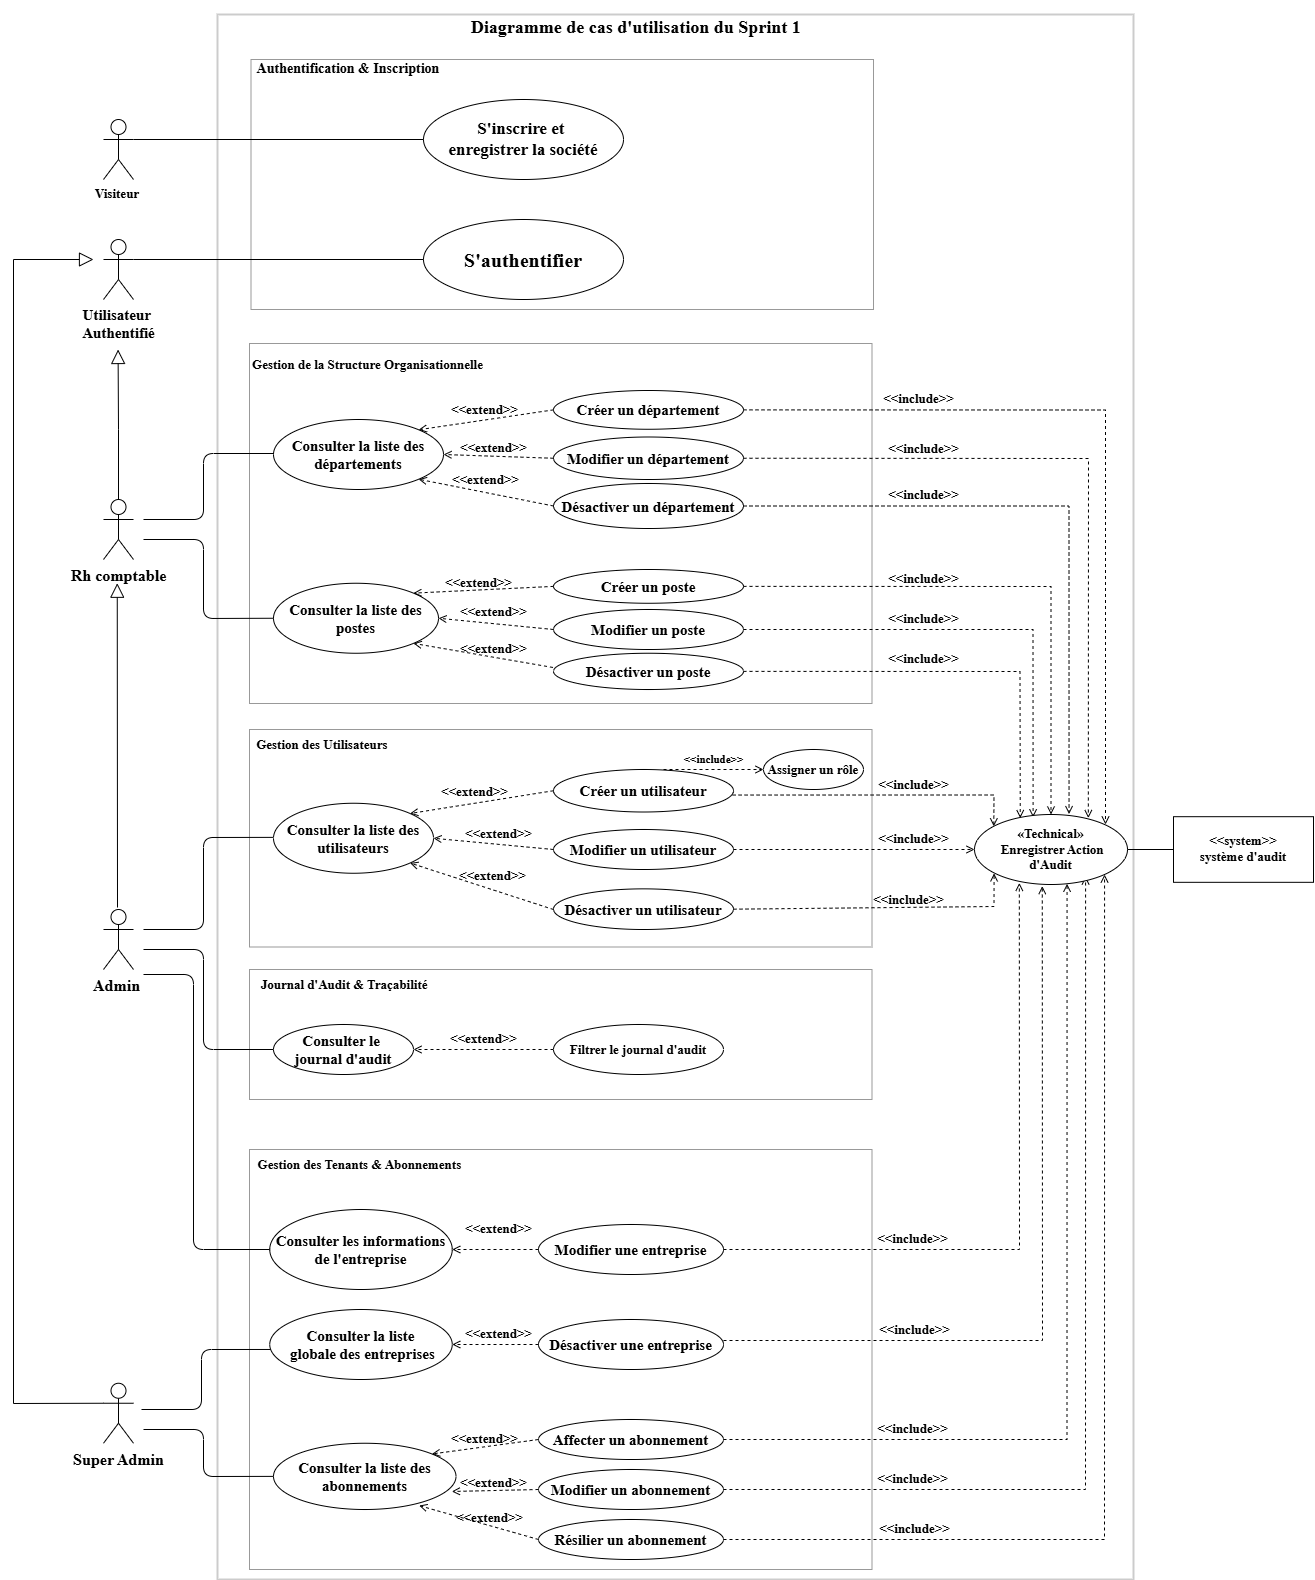
\includegraphics[width=0.95\textwidth]{use-case-sp1}
    \caption{Diagramme de cas d'utilisation raffiné du Sprint~1}
    \label{fig:use-case-s1}
\end{figure}

Le diagramme s'organise comme suit :

\medskip
\noindent\textbf{Relations structurelles UML :}
Le cas d'utilisation \og{}S'authentifier\fg{} est en relation \texttt{<<include>>} 
avec l'ensemble des cas d'utilisation protégés, matérialisant la précondition d'accès 
obligatoire. La vérification 2FA étend (\texttt{<<extend>>}) le flux nominal 
d'authentification pour les comptes Super Admin et Admin. Une relation de 
généralisation unit les acteurs \textsc{Admin} et \textsc{RH}~: l'Admin hérite de 
tous les cas d'utilisation du RH et dispose en sus de ses propres prérogatives.
\medskip
\noindent\textbf{Responsabilités par acteur :}

\begin{itemize}[label=\textbullet, leftmargin=0.6cm]

  \item \textbf{Visiteur :} Unique acteur non authentifié. Déclenche le cas 
  d'utilisation \og{}S'inscrire et enregistrer la société\fg{}, qui initie 
  automatiquement le Tenant Provisioning (création du schéma PostgreSQL dédié). 
  À l'issue de ce flux, le Visiteur acquiert le rôle Admin Entreprise.

  \item \textbf{Utilisateur (rôle générique) :} Regroupe tout compte authentifié, 
  quel que soit son rôle. Il peut s'authentifier, activer la 2FA et gérer son profil.

  \item \textbf{Admin Entreprise :} Gère les informations légales de la société, 
  administre les comptes utilisateurs (création directe ou invitation par e-mail), 
  configure la structure organisationnelle et consulte le journal d'audit.

  \item \textbf{Super Admin :} Supervise les entreprises clientes et pilote les 
  abonnements SaaS (affectation, modification, résiliation).

  \item \textbf{RH Comptable :} Dans le périmètre du Sprint~1, intervient 
  uniquement dans la définition de la structure organisationnelle (départements 
  et postes).

\end{itemize}

% -----------------------------------------------------------
\subsection{Description textuelle des cas d'utilisation}
% -----------------------------------------------------------
Les descriptions textuelles détaillent les préconditions et scénarios (nominaux et 
alternatifs) des cas d'utilisation. Elles servent de référence contractuelle pour 
valider les fonctionnalités du sprint avec le Product Owner.

% -----------------------------------------------------------
\subsubsection{Cas d'utilisation 1 : S'authentifier}
% -----------------------------------------------------------
Le tableau~\ref{tab:uc_authentification} présente la description textuelle détaillée 
du cas d'utilisation \og{}S'authentifier\fg{}.

\vspace{0.2cm}
\begin{xltabular}{\textwidth}{|l|X|}
    \hline
    \rowcolor[gray]{0.9} \textbf{Élément} & \textbf{Description} \\ \hline
    \endfirsthead
    \hline
    \rowcolor[gray]{0.9} \textbf{Élément} & \textbf{Description} \\ \hline
    \endhead
    \hline
    \endfoot
    \endfoot
    \endlastfoot
    \textbf{Titre} & S'authentifier \\ \hline
    \textbf{Acteur principal} & Utilisateur (Admin, RH Comptable, Super Admin, Employé) \\ \hline
    \textbf{Préconditions} & L'utilisateur dispose d'un compte actif, non suspendu, 
    et de ses identifiants de connexion (e-mail et mot de passe). \\ \hline
    \textbf{Postconditions} & Un token JWT est généré et transmis au client. 
    L'utilisateur est redirigé vers le tableau de bord correspondant à son rôle. \\ \hline
    \textbf{Scénario principal} &
    \begin{enumerate}[nosep, leftmargin=*]
        \item L'utilisateur accède à l'interface de connexion.
        \item Il saisit son adresse e-mail et son mot de passe.
        \item Le système vérifie les identifiants et contrôle le statut du compte 
              (actif / suspendu).
        \item Un token JWT signé (durée de vie limitée) est généré et retourné 
              au client Angular.
        \item Le système identifie le rôle et le tenant de l'utilisateur depuis 
              le payload du token.
        \item L'utilisateur est redirigé vers le tableau de bord correspondant 
              à son rôle (\texttt{ROLE\_SUPER\_ADMIN}, \texttt{ROLE\_ADMIN}, 
              \texttt{ROLE\_RH\_COMPTABLE} ou \texttt{ROLE\_EMPLOYE}).
    \end{enumerate} \\ \hline
    \textbf{Scénarios alternatifs}
    & \textbf{A1 : Identifiants incorrects} $\rightarrow$ Le système affiche un 
      message d'erreur générique et invite à une nouvelle saisie (sans préciser 
      si c'est l'e-mail ou le mot de passe qui est erroné, pour éviter 
      l'énumération de comptes). \\ \cline{2-2}
    & \textbf{A2 : Compte suspendu} $\rightarrow$ Le système informe l'utilisateur 
      que son accès a été désactivé et l'invite à contacter l'administrateur. \\ \cline{2-2}
    & \textbf{A3 : Authentification 2FA requise} $\rightarrow$ Pour les comptes 
      Super Admin et Admin, après validation du mot de passe, le système exige 
      la saisie d'un code TOTP (Time-based One-Time Password) généré par 
      l'application d'authentification de l'utilisateur. \\ \hline
      \caption{Description textuelle du cas d'utilisation S'authentifier}
    \label{tab:uc_authentification}
\end{xltabular}

% -----------------------------------------------------------
\subsubsection{Cas d'utilisation 2 : S'inscrire et enregistrer la société}
% -----------------------------------------------------------
Le tableau~\ref{tab:uc_inscription} présente la description textuelle détaillée du 
cas d'utilisation \og{}S'inscrire et enregistrer la société\fg{}.

\vspace{0.2cm}
\begin{xltabular}{\textwidth}{|l|X|}
    
    \hline
    \rowcolor[gray]{0.9} \textbf{Élément} & \textbf{Description} \\ \hline
    \endfirsthead
    \hline
    \rowcolor[gray]{0.9} \textbf{Élément} & \textbf{Description} \\ \hline
    \endhead
    \hline
    \endfoot
    \endfoot
    \endlastfoot

    \textbf{Titre} & S'inscrire et enregistrer la société \\ \hline
    \textbf{Acteur principal} & Visiteur \\ \hline
    \textbf{Préconditions} & Le visiteur ne possède pas de compte PaieZone. 
    L'adresse e-mail et le matricule fiscal de la société renseignés ne sont 
    pas déjà enregistrés dans le système. \\ \hline
    \textbf{Postconditions} & Un schéma PostgreSQL isolé est créé pour la société 
    (Tenant Provisioning). Les migrations Liquibase sont appliquées automatiquement. 
    Le visiteur devient l'Administrateur responsable de cet espace et son compte 
    est activé. Un e-mail de confirmation est envoyé. \\ \hline
    \textbf{Scénario principal} &
    \begin{enumerate}[nosep, leftmargin=*]
        \item Le visiteur accède au formulaire d'inscription.
        \item Il renseigne ses informations personnelles (nom, prénom, e-mail, 
              mot de passe) et les informations légales de sa société 
              (raison sociale, matricule fiscal, adresse).
        \item Le système valide les données transmises (format, unicité).
        \item Un schéma PostgreSQL dédié est créé pour la société et les migrations 
              Liquibase sont appliquées, initialisant la structure de la base de 
              données du tenant.
        \item Un compte Administrateur est créé et associé à la société.
        \item Un e-mail de confirmation d'inscription est envoyé à l'adresse fournie.
        \item Le visiteur (désormais Administrateur) est redirigé vers la page 
              de connexion.
    \end{enumerate} \\ \hline
    \textbf{Scénarios alternatifs}
    & \textbf{A1 : Adresse e-mail déjà utilisée} $\rightarrow$ Le système affiche 
      un message d'erreur indiquant que l'e-mail est déjà associé à un compte 
      existant. \\ \cline{2-2}
    & \textbf{A2 : Données invalides} $\rightarrow$ Le système affiche les erreurs 
      de validation spécifiques sur les champs concernés. \\ \cline{2-2}
    & \textbf{A3 : Matricule fiscal déjà enregistré} $\rightarrow$ Le système 
      bloque la création et indique que cette société est déjà inscrite sur 
      la plateforme. 
      \\ \hline
    \caption{Description textuelle du cas d'utilisation S'inscrire et enregistrer la société}
    \label{tab:uc_inscription}
\end{xltabular}

% -----------------------------------------------------------
\subsubsection{Cas d'utilisation 3 : Gérer les utilisateurs}
% -----------------------------------------------------------
Le tableau~\ref{tab:uc_gestion_utilisateurs} présente la description textuelle 
détaillée du cas d'utilisation \og{}Gérer les utilisateurs\fg{}.

\vspace{0.2cm}
\begin{xltabular}{\textwidth}{|l|X|}
    
    \hline
    \rowcolor[gray]{0.9} \textbf{Élément} & \textbf{Description} \\ \hline
    \endfirsthead
    \hline
    \rowcolor[gray]{0.9} \textbf{Élément} & \textbf{Description} \\ \hline
    \endhead
    \hline
    \endfoot
    \endfoot
    \endlastfoot

    \textbf{Titre} & Gérer les utilisateurs (Créer / Inviter / Modifier / 
    Désactiver) \\ \hline
    \textbf{Acteur principal} & Admin \\ \hline
    \textbf{Préconditions} & L'Administrateur est authentifié et dispose des droits 
    de gestion des utilisateurs sur son tenant. \\ \hline
    \textbf{Postconditions} & L'utilisateur ciblé est créé, invité, modifié ou 
    désactivé. L'action est enregistrée automatiquement dans le journal d'audit 
    (interception AOP). \\ \hline
    \textbf{Scénario principal} &
    \begin{enumerate}[nosep, leftmargin=*]
        \item L'Administrateur accède à l'interface de gestion des utilisateurs.
        \item Il consulte la liste paginée des utilisateurs de sa société.
        \item Il sélectionne l'action souhaitée :
        \begin{itemize}[nosep, leftmargin=*]
            \item \textbf{Création directe :} renseigne les informations 
                  (nom, e-mail, rôle) et confirme ; un compte activé est créé.
            \item \textbf{Invitation par e-mail :} saisit l'e-mail et le rôle ; 
                  le système génère un token d'invitation (validité 7~jours) et 
                  envoie un lien d'activation ; le compte reste inactif jusqu'à 
                  l'acceptation.
            \item \textbf{Modification :} met à jour les informations ou le rôle 
                  d'un compte existant.
            \item \textbf{Désactivation :} révoque immédiatement les droits d'accès.
        \end{itemize}
        \item Le système valide les données et applique les changements en base 
              de données ; l'action est tracée automatiquement dans le journal 
              d'audit (horodatage, identité de l'auteur, valeurs avant/après).
        \item Un message de confirmation est affiché.
    \end{enumerate} \\ \hline
    \textbf{Scénarios alternatifs}
    & \textbf{A1 : Utilisateur introuvable} $\rightarrow$ Le système affiche 
      un message d'erreur. \\ \cline{2-2}
    & \textbf{A2 : Droits insuffisants} $\rightarrow$ Exception 403 levée 
      par Spring Security. \\ \cline{2-2}
    & \textbf{A3 : E-mail déjà utilisé} $\rightarrow$ Le système bloque 
      l'enregistrement. \\ \cline{2-2}
    & \textbf{A4 : Token d'invitation expiré} $\rightarrow$ Le système invalide 
      le lien et invite l'utilisateur à contacter l'administrateur pour 
      un renvoi.
    \\ \hline
    \caption{Description textuelle du cas d'utilisation Gérer les utilisateurs}
    \label{tab:uc_gestion_utilisateurs} 
\end{xltabular}
% ============================================================
\section{Conception du premier Sprint}
\label{sec:s1-conception}
% ============================================================
La conception technique de PaieZone~RH matérialise les besoins métiers à travers des 
modèles structurants guidant le développement. Cette section s'articule autour de deux 
axes complémentaires~: le diagramme de classes, qui décrit l'architecture statique des 
entités, et les diagrammes de séquences, qui modélisent la dynamique des interactions.

% ============================================================
\subsection{Diagramme de classes}
% ============================================================
Le diagramme de classes modélise l'architecture statique du système. Il définit la 
structure des données en précisant les entités, leurs attributs et les relations de 
dépendance qui les unissent, offrant ainsi une vue d'ensemble de l'organisation logique 
de PaieZone.

\begin{figure}[htbp]
    \centering
    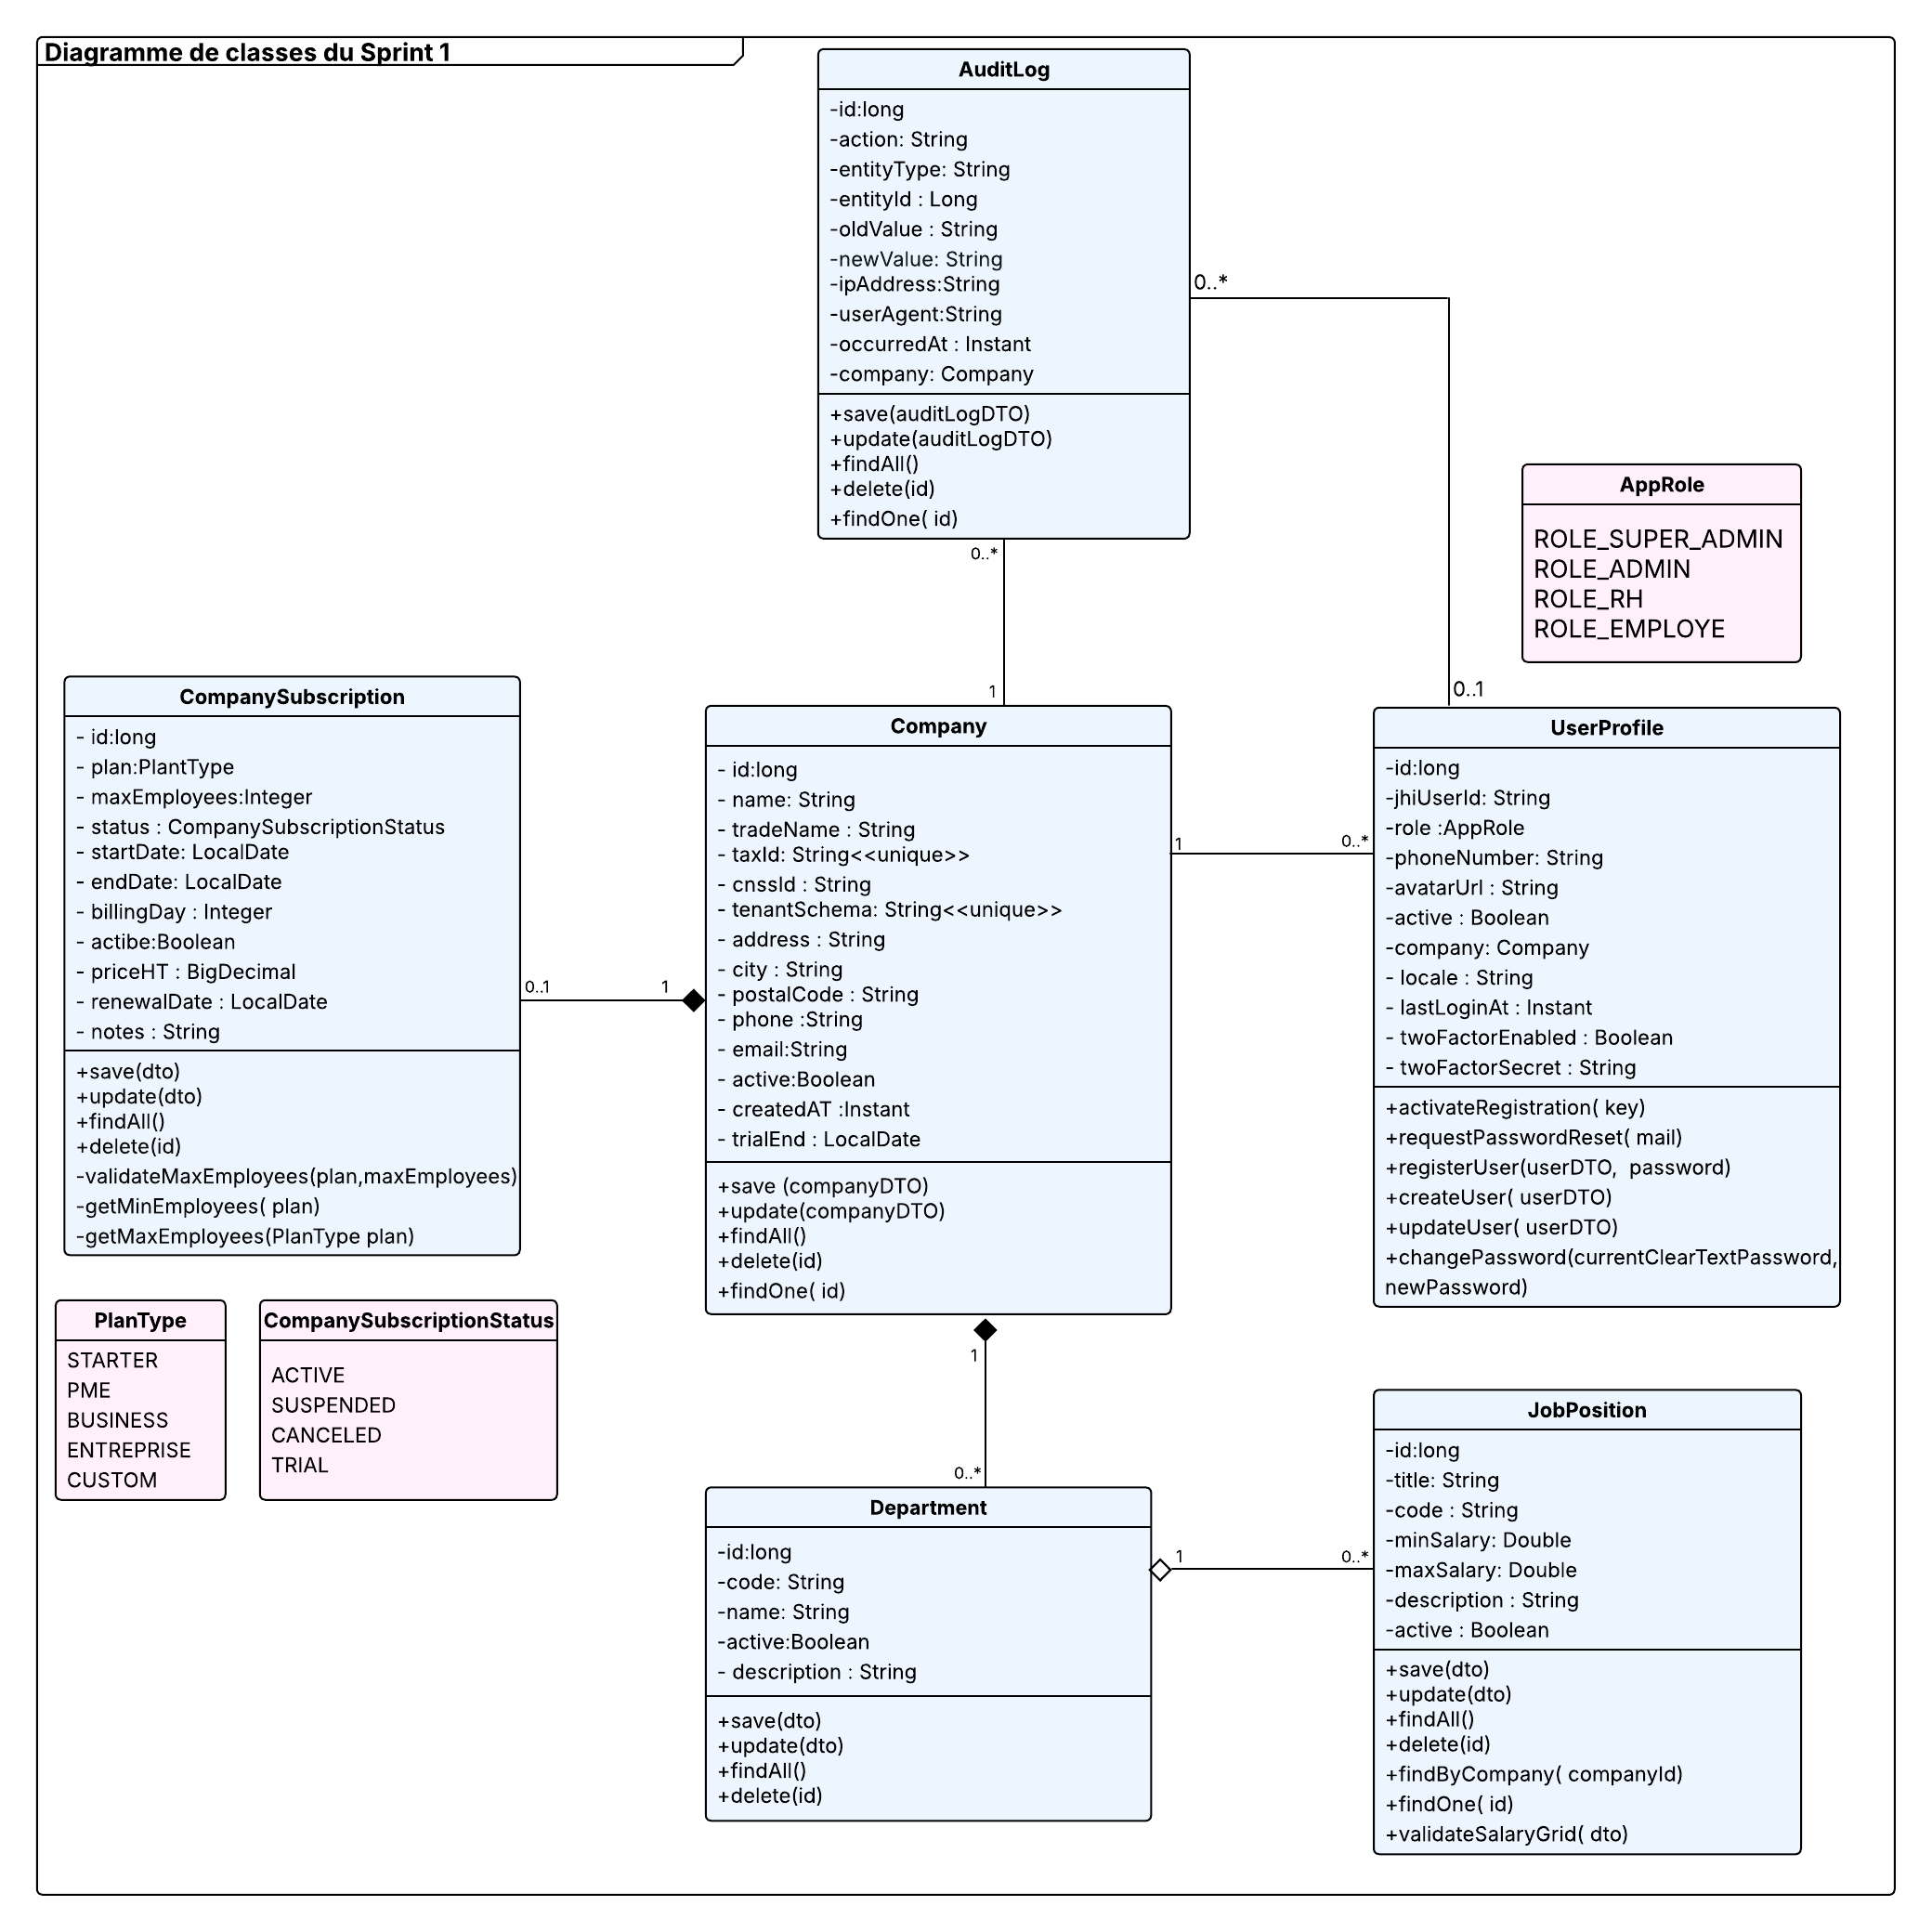
\includegraphics[width=0.99\textwidth]{classes-sprint1}
    \caption{Diagramme de classes du Sprint~1}
    \label{fig:classes-sprint1}
\end{figure}
La structure statique des données pour ce premier sprint est modélisée par le diagramme de classes illustré en Figure~\ref{fig:classes-sprint1}. Ce schéma expose les entités fondamentales de PaieZone ainsi que les liens logiques qui les unissent, constituant ainsi le socle du modèle de données applicatif. Les composants majeurs et leurs interactions se présentent comme suit :
\begin{itemize}[label=\textbullet, leftmargin=0.6cm]

    \item \textbf{Company~:} représente un tenant (entreprise cliente). Elle porte 
    l'identifiant fiscal (\texttt{taxId}), le schéma PostgreSQL dédié 
    (\texttt{tenantSchema}) et la référence à son abonnement SaaS 
    (\texttt{CompanySubscription}).

    \item \textbf{CompanySubscription~:} modélise le plan souscrit par l'entreprise 
    (type, statut, dates de début/fin). Elle est liée à \texttt{Company} par une 
    association~1-1.

    \item \textbf{User~:} entité JHipster standard gérant l'authentification (login, 
    password hashé, authorities). Elle est liée à \texttt{UserProfile} par une 
    association~1-1.

    \item \textbf{UserProfile~:} étend \texttt{User} avec les informations métier 
    (nom, prénom, e-mail professionnel) et rattache l'utilisateur à une 
    \texttt{Company}.

    \item \textbf{Department~:} département de l'entreprise, rattaché à 
    \texttt{Company} par une association de composition.

    \item \textbf{JobPosition~:} poste de travail rattaché à un \texttt{Department}. 
    Chaque employé (Sprint~2) sera associé à un \texttt{JobPosition}.

    \item \textbf{AuditLog~:} enregistre chaque action sensible avec l'action, le 
    type et l'identifiant de l'entité cible, les valeurs avant/après, l'adresse IP 
    et l'horodatage.
\end{itemize}

% ============================================================
\subsection{Diagrammes de séquences}
% ============================================================
Le diagramme de séquences illustre la dynamique du système en détaillant les 
interactions chronologiques entre les objets. Il permet de visualiser le flux de 
messages échangés pour réaliser un cas d'utilisation spécifique, précisant ainsi le 
comportement temporel des composants.
\newpage

% -----------------------------------------------------------
\subsubsection{Diagramme de séquence : Authentification}
% -----------------------------------------------------------
La figure~\ref{fig:seq-auth} illustre le flux d'authentification, 
couvrant la validation des identifiants, la génération du token JWT et la 
redirection vers le tableau de bord selon le rôle de l'utilisateur.
\vspace{1cm}
\begin{figure}[htbp]
    \centering
    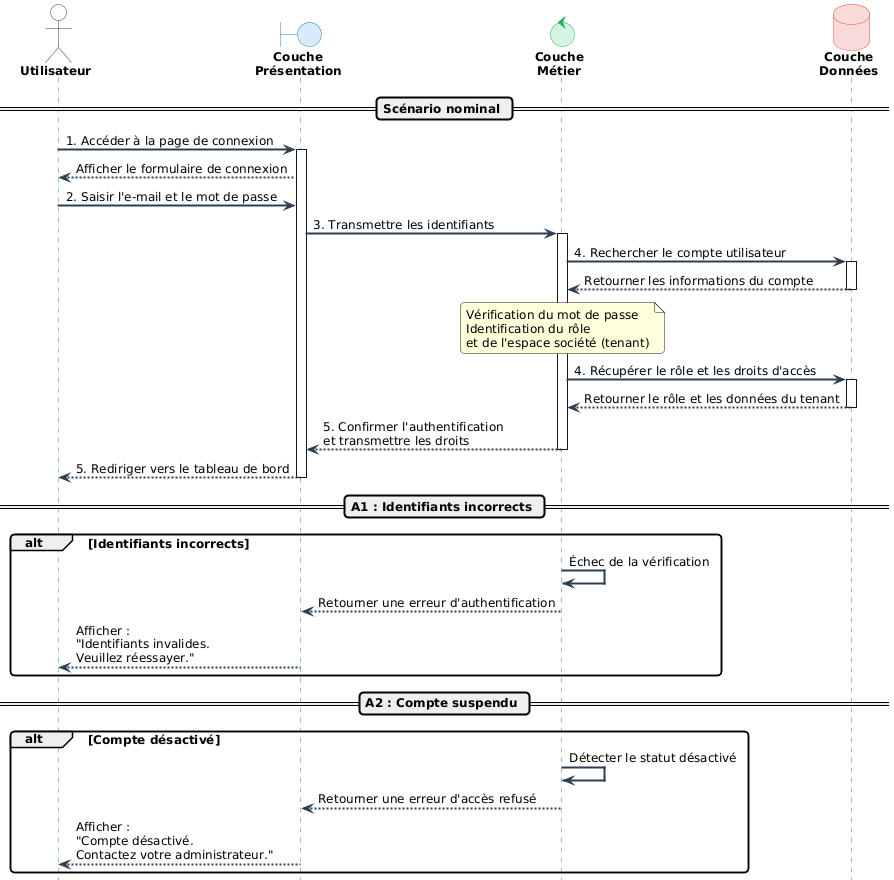
\includegraphics[width=0.99\textwidth]{seq-sp1-uc1.png}
    \caption{Diagramme de séquence — Authentification}
    \label{fig:seq-auth}
\end{figure}
\newpage

% -----------------------------------------------------------
\subsubsection{Diagramme de séquence : Création d'un utilisateur 
avec enregistrement d'audit}
% -----------------------------------------------------------
La figure~\ref{fig:seq-create-user} illustre le flux de création d'un utilisateur, incluant le déclenchement automatique de l'enregistrement dans le 
journal d'audit via l'interception AOP Spring. Le flux modélisé couvre~:

\vspace{1cm}

\begin{figure}[htbp]
    \centering
    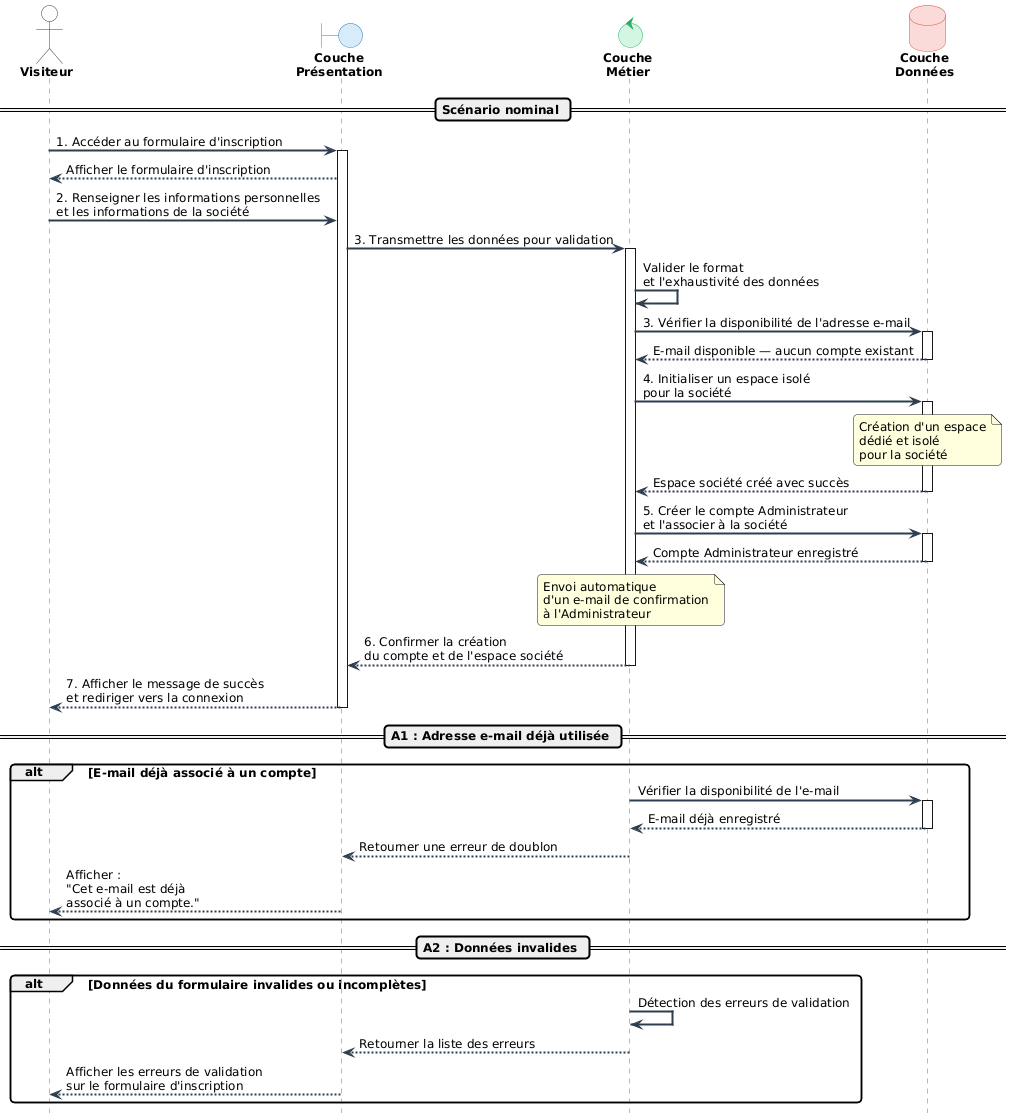
\includegraphics[width=0.99\textwidth]{seq-sp1-uc2.png}
    \caption{Diagramme de séquence — Création d'un utilisateur avec 
    enregistrement d'audit}
    \label{fig:seq-create-user}
\end{figure}

% ============================================================
\section{Réalisation du premier Sprint}
\label{sec:s1-realisation}
% ============================================================
Cette section détaille les réalisations concrètes du premier sprint, marquant le 
passage des spécifications à une solution logicielle fonctionnelle. Les travaux ont 
porté sur la mise en place de l'infrastructure technique, l'implémentation du socle 
de sécurité et le développement des premières interfaces utilisateurs. Cette étape 
matérialise la validation des User Stories prioritaires, notamment la gestion des 
accès et l'isolation des données, posant ainsi les fondations robustes de la 
plateforme PaieZone.

% -----------------------------------------------------------
\subsection{Inscription et initialisation de l'espace société}
% -----------------------------------------------------------
Le flux d'inscription de PaieZone est conçu pour permettre à un nouveau client 
(Visiteur) de créer simultanément son compte administrateur et l'espace isolé de 
sa société en une seule démarche guidée.

\begin{figure}[htbp]
    \centering
    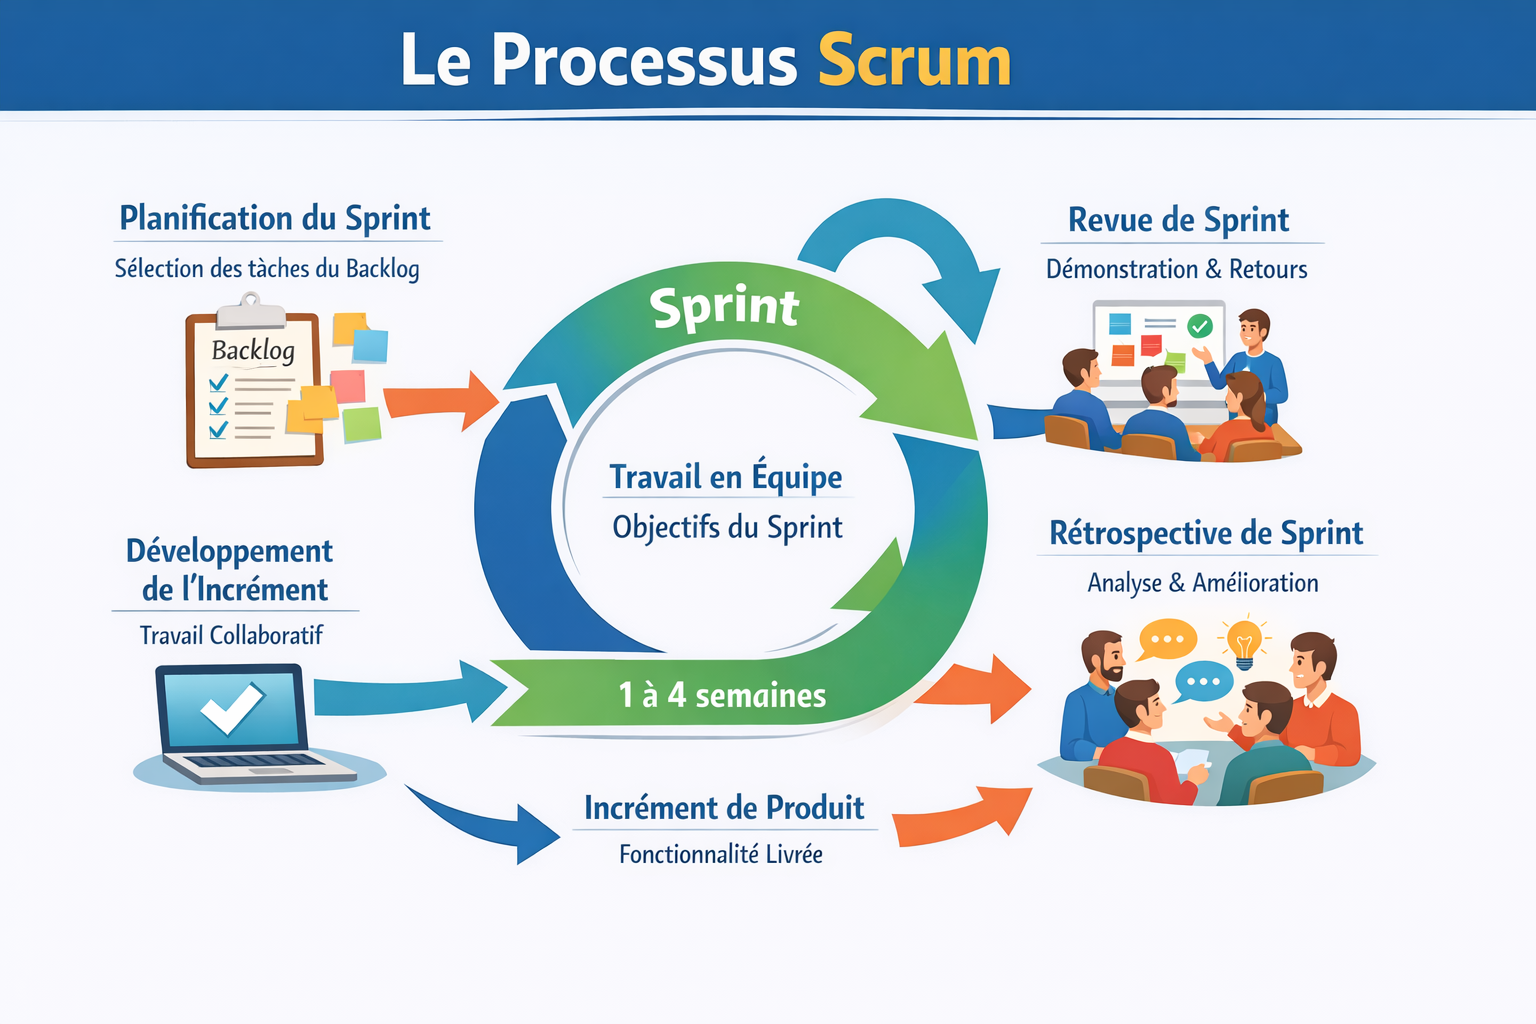
\includegraphics[width=0.7\textwidth]{scrum.png}
    \caption{Formulaire d'inscription — Informations personnelles et informations 
    de la société}
    \label{fig:ui-inscription}
\end{figure}

La figure~\ref{fig:ui-inscription} illustre le formulaire d'inscription, 
regroupant les données personnelles de l'administrateur et les informations légales 
de l'entreprise. La validation de ce formulaire déclenche automatiquement le 
provisionnement d'un schéma PostgreSQL dédié et l'application des migrations 
Liquibase, garantissant l'isolation complète des données de la société au sein de 
la base de données.

% -----------------------------------------------------------
\subsection{Authentification et accès}
% -----------------------------------------------------------
L'authentification constitue le point d'entrée unique de la plateforme PaieZone. 
Le système implémente un mécanisme de connexion sécurisé basé sur le standard JWT 
(JSON Web Token), complété par une redirection intelligente vers le tableau de bord 
correspondant au rôle de l'utilisateur connecté.

\begin{figure}[htbp]
    \centering
    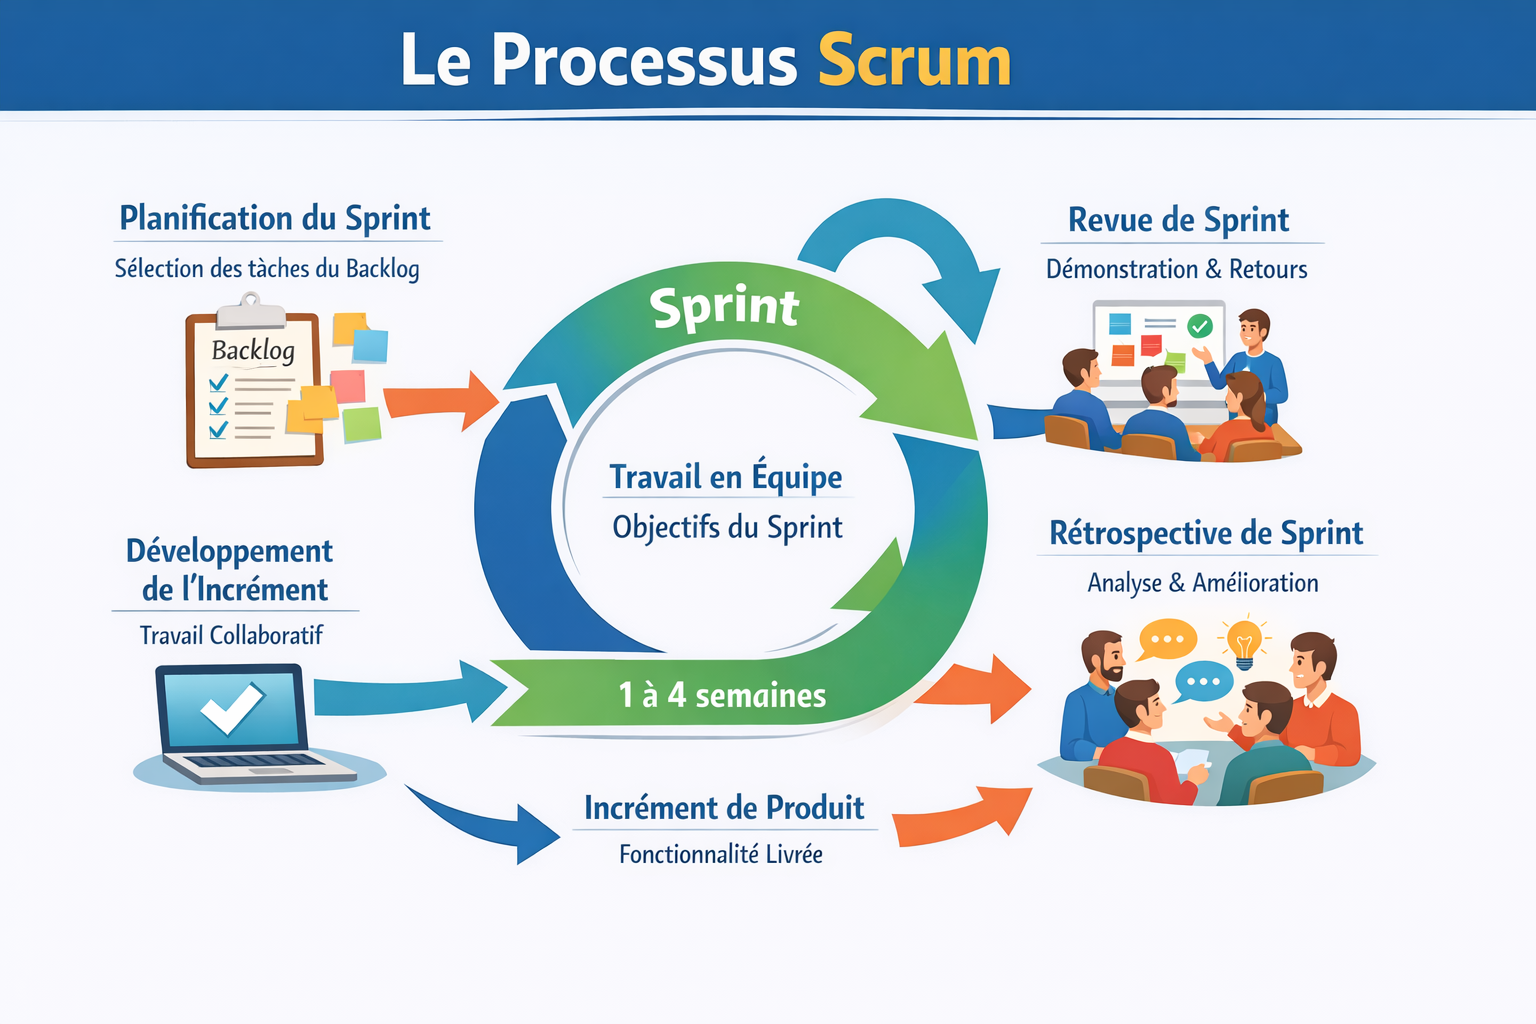
\includegraphics[width=0.75\textwidth]{scrum.png}
    \caption{Page de connexion de \pz}
    \label{fig:ui-login}
\end{figure}

La figure~\ref{fig:ui-login} présente la page de connexion d. Le formulaire 
collecte l'adresse e-mail et le mot de passe de l'utilisateur. En cas d'échec 
d'authentification, un message d'erreur générique est affiché, sans préciser si 
c'est l'e-mail ou le mot de passe qui est erroné, conformément aux bonnes pratiques 
de sécurité.

\begin{figure}[htbp]
    \centering
    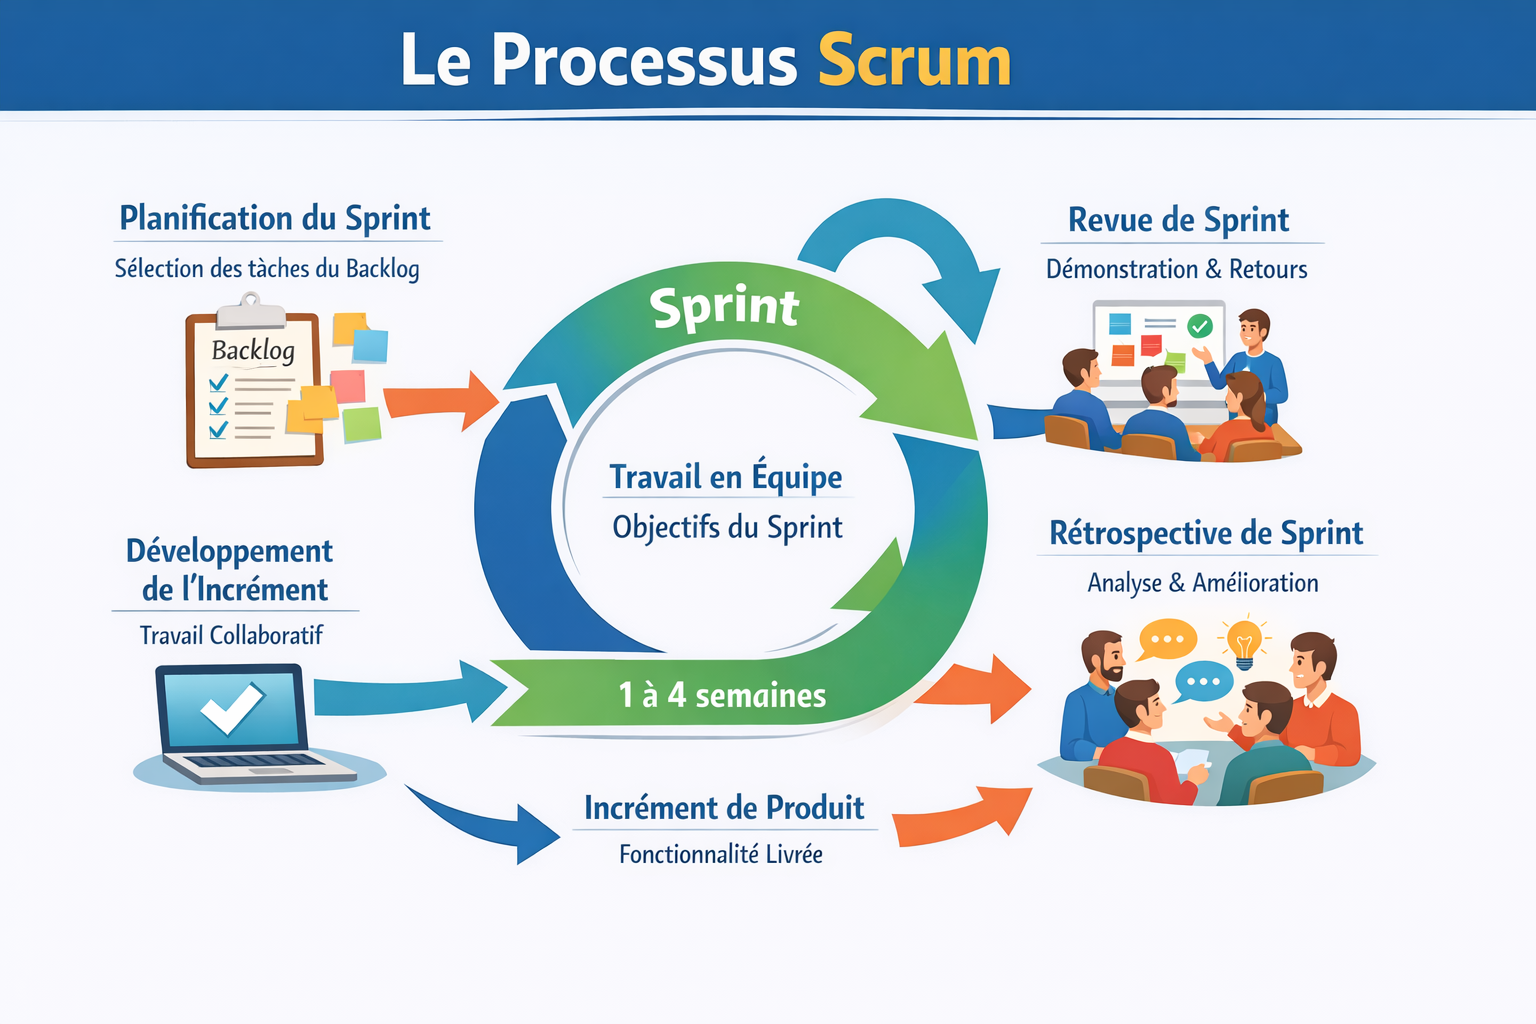
\includegraphics[width=0.75\textwidth]{scrum.png}
    \caption{Tableau de bord — Vue SuperAdmin après authentification}
    \label{fig:ui-dashboard-Superadmin}
\end{figure}

\begin{figure}[htbp]
    \centering
    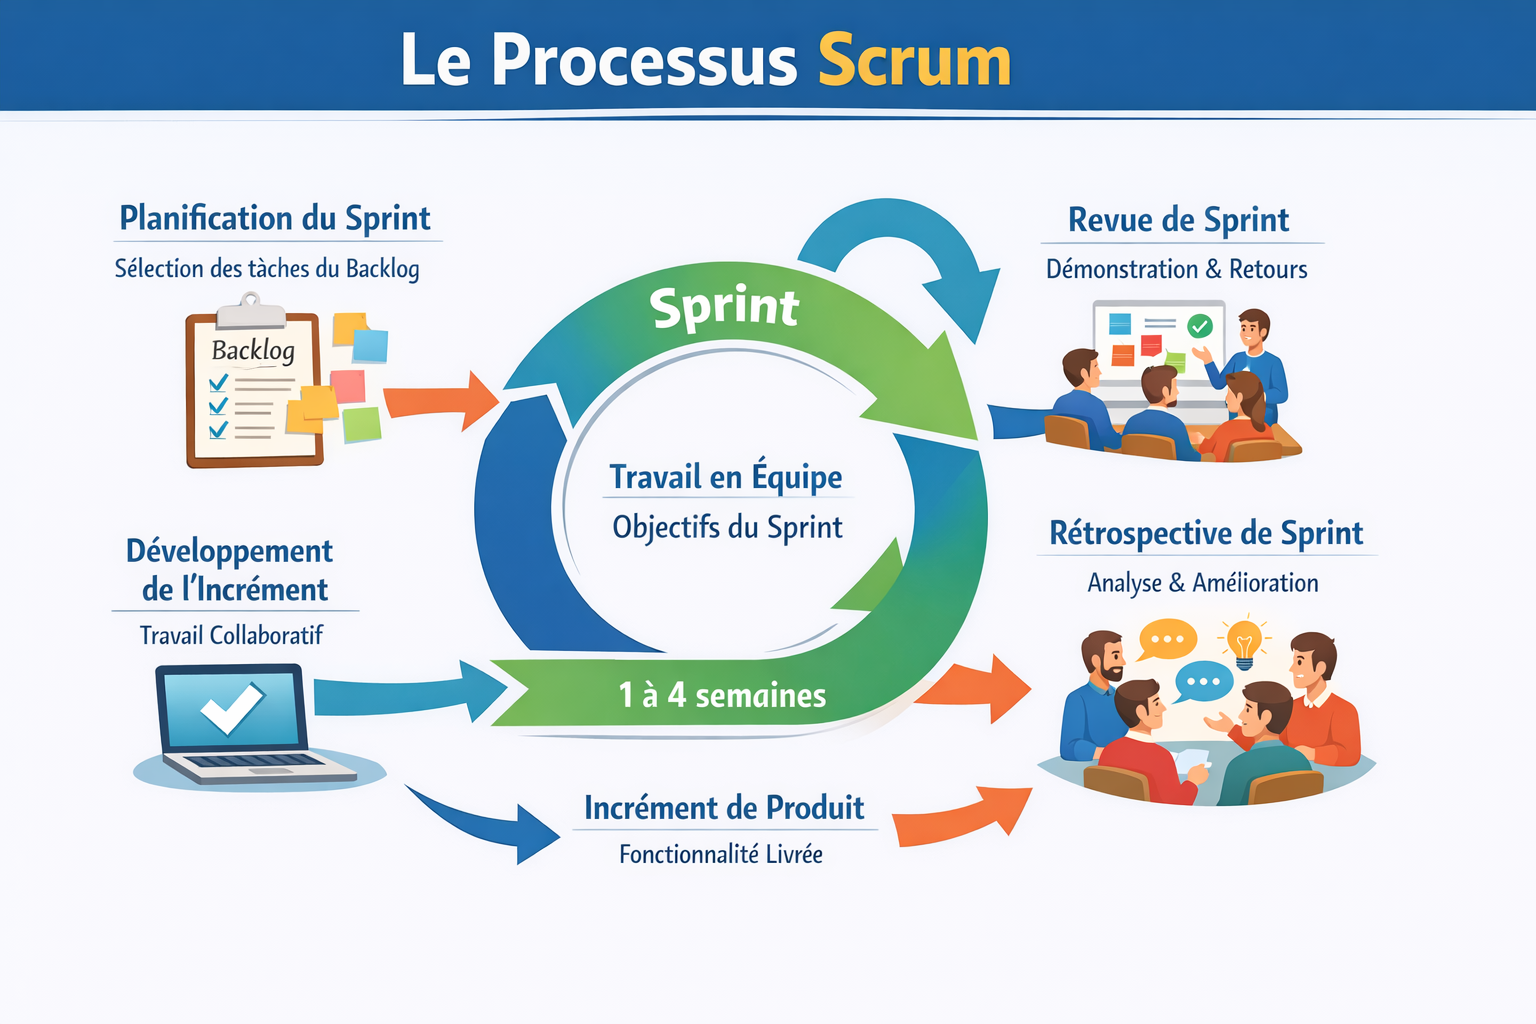
\includegraphics[width=0.75\textwidth]{scrum.png}
    \caption{Tableau de bord — Vue Administrateur après authentification}
    \label{fig:ui-dashboard-admin}
\end{figure}

\newpage

\begin{figure}[htbp]
    \centering
    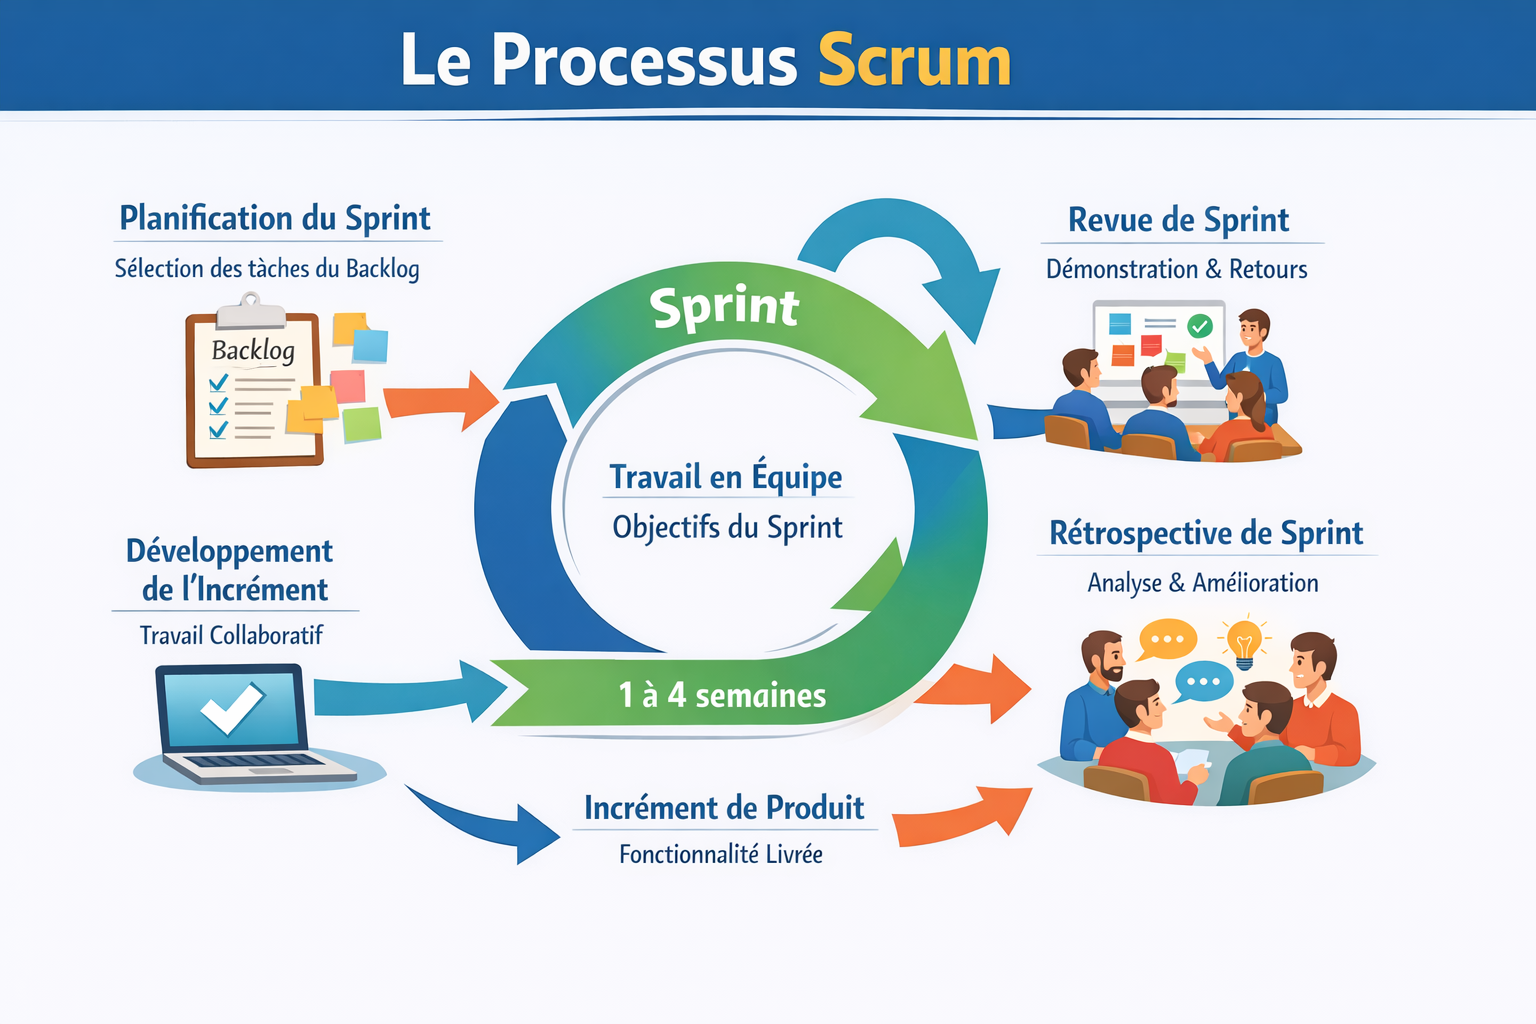
\includegraphics[width=0.75\textwidth]{scrum.png}
    \caption{Tableau de bord — Vue Employé après authentification}
    \label{fig:ui-dashboard-employe}
\end{figure}

\begin{figure}[htbp]
    \centering
    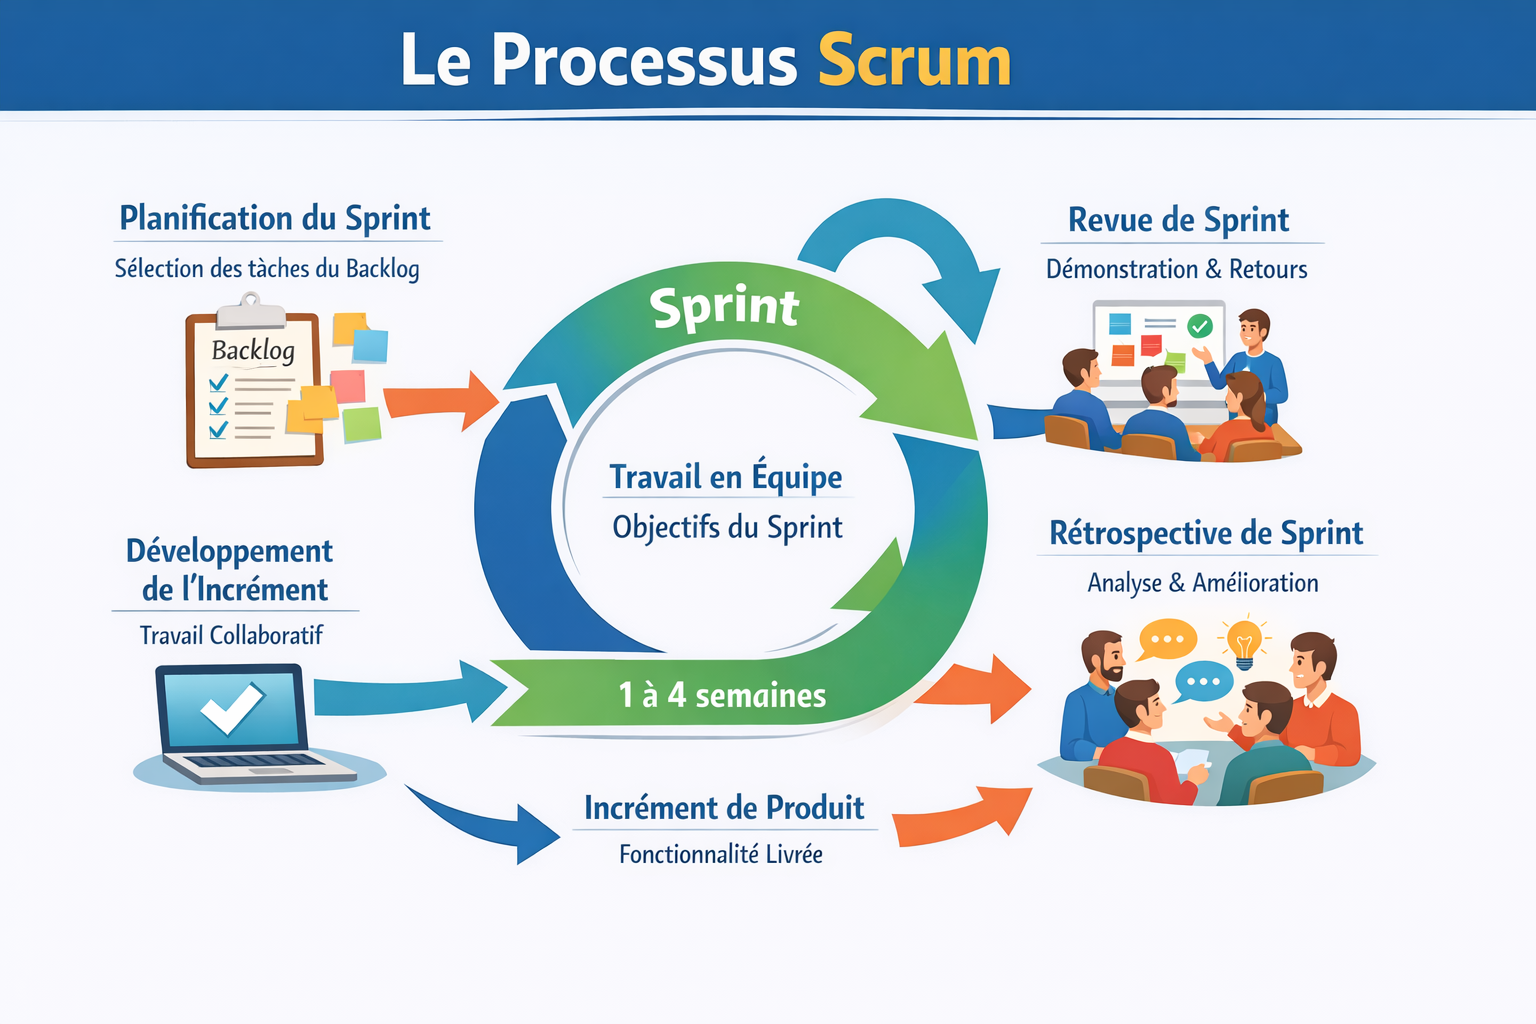
\includegraphics[width=0.75\textwidth]{scrum.png}
    \caption{Tableau de bord — Vue RH après authentification}
    \label{fig:ui-dashboard-rh}
\end{figure}

\newpage
Les figures \ref{fig:ui-dashboard-admin} à \ref{fig:ui-dashboard-rh} illustrent la redirection basée sur le modèle RBAC. Une fois authentifié, l'utilisateur est orienté vers un tableau de bord spécifique à son rôle (Super Admin, Admin, RH Comptable ou Employé), garantissant un accès sécurisé aux seuls modules autorisés.

% -----------------------------------------------------------
\subsection{Gestion des utilisateurs}
% -----------------------------------------------------------
Le module de gestion des utilisateurs, pilier central du premier sprint, permet à 
l'Administrateur de piloter l'ensemble des comptes collaborateurs (création, 
invitation, modification et désactivation).

\begin{figure}[htbp]
    \centering
    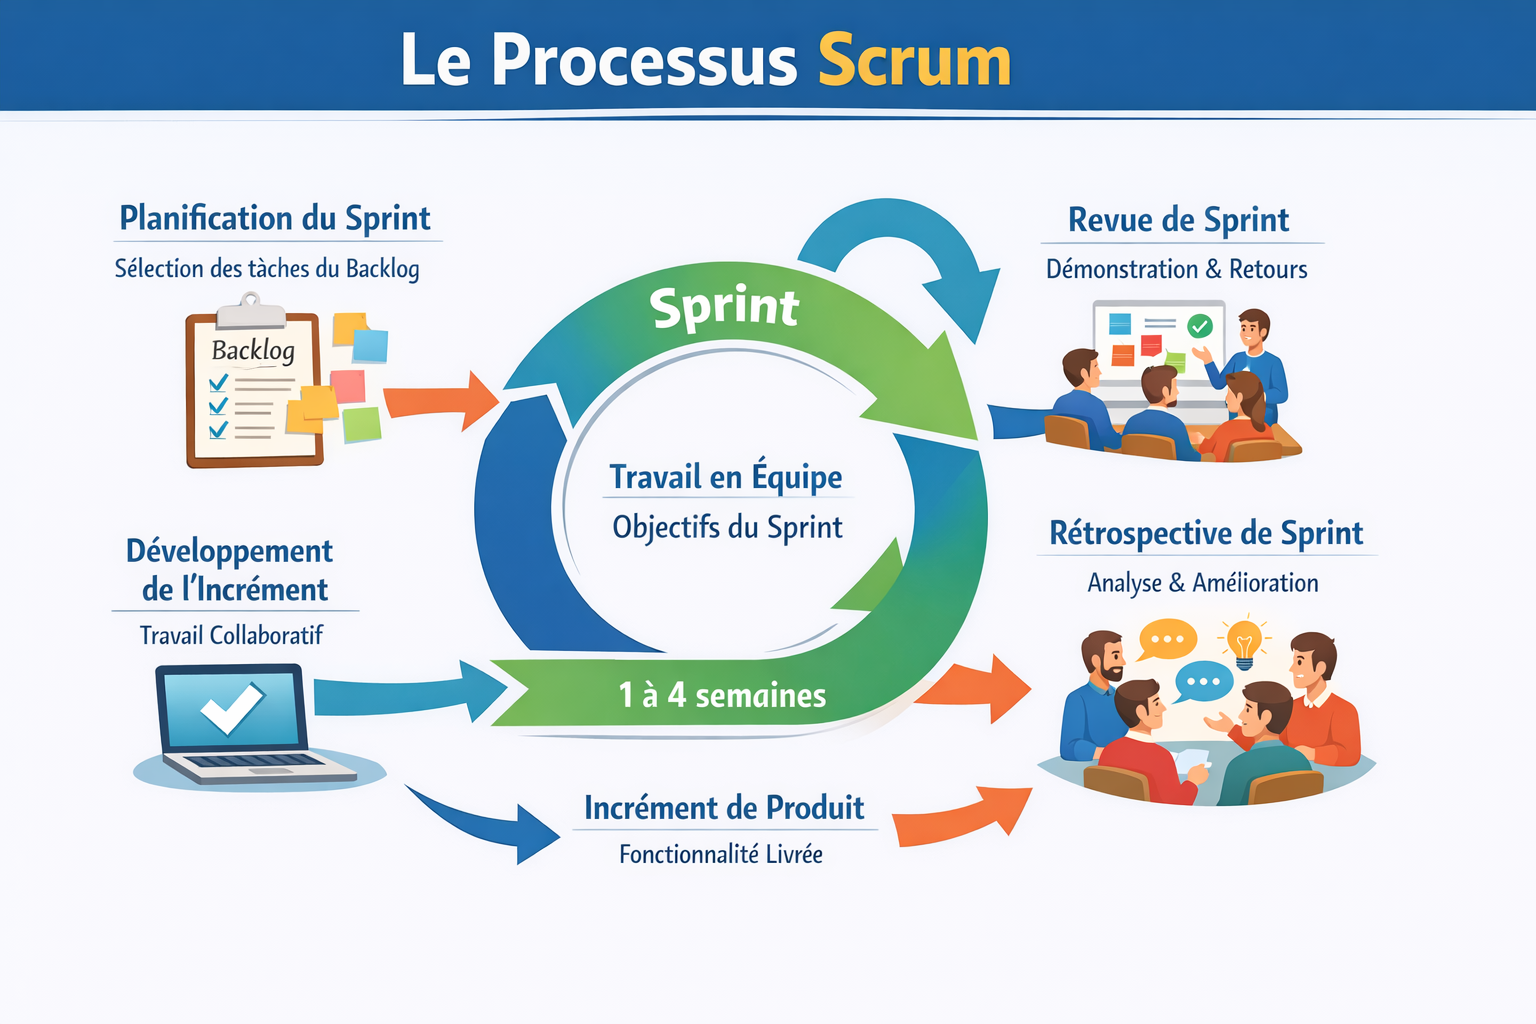
\includegraphics[width=0.70\textwidth]{scrum.png}
    \caption{Liste des utilisateurs}
    \label{fig:ui-users-list}
\end{figure}

\newpage
La figure~\ref{fig:ui-users-list} illustre l'interface de consultation, où les 
utilisateurs sont listés avec leurs informations clés~: identité, rôle et statut. 
Pour optimiser l'expérience de gestion, cette table intègre des fonctions de 
recherche et de pagination, facilitant la navigation au sein des effectifs de 
l'entreprise.

\begin{figure}[htbp]
    \centering
    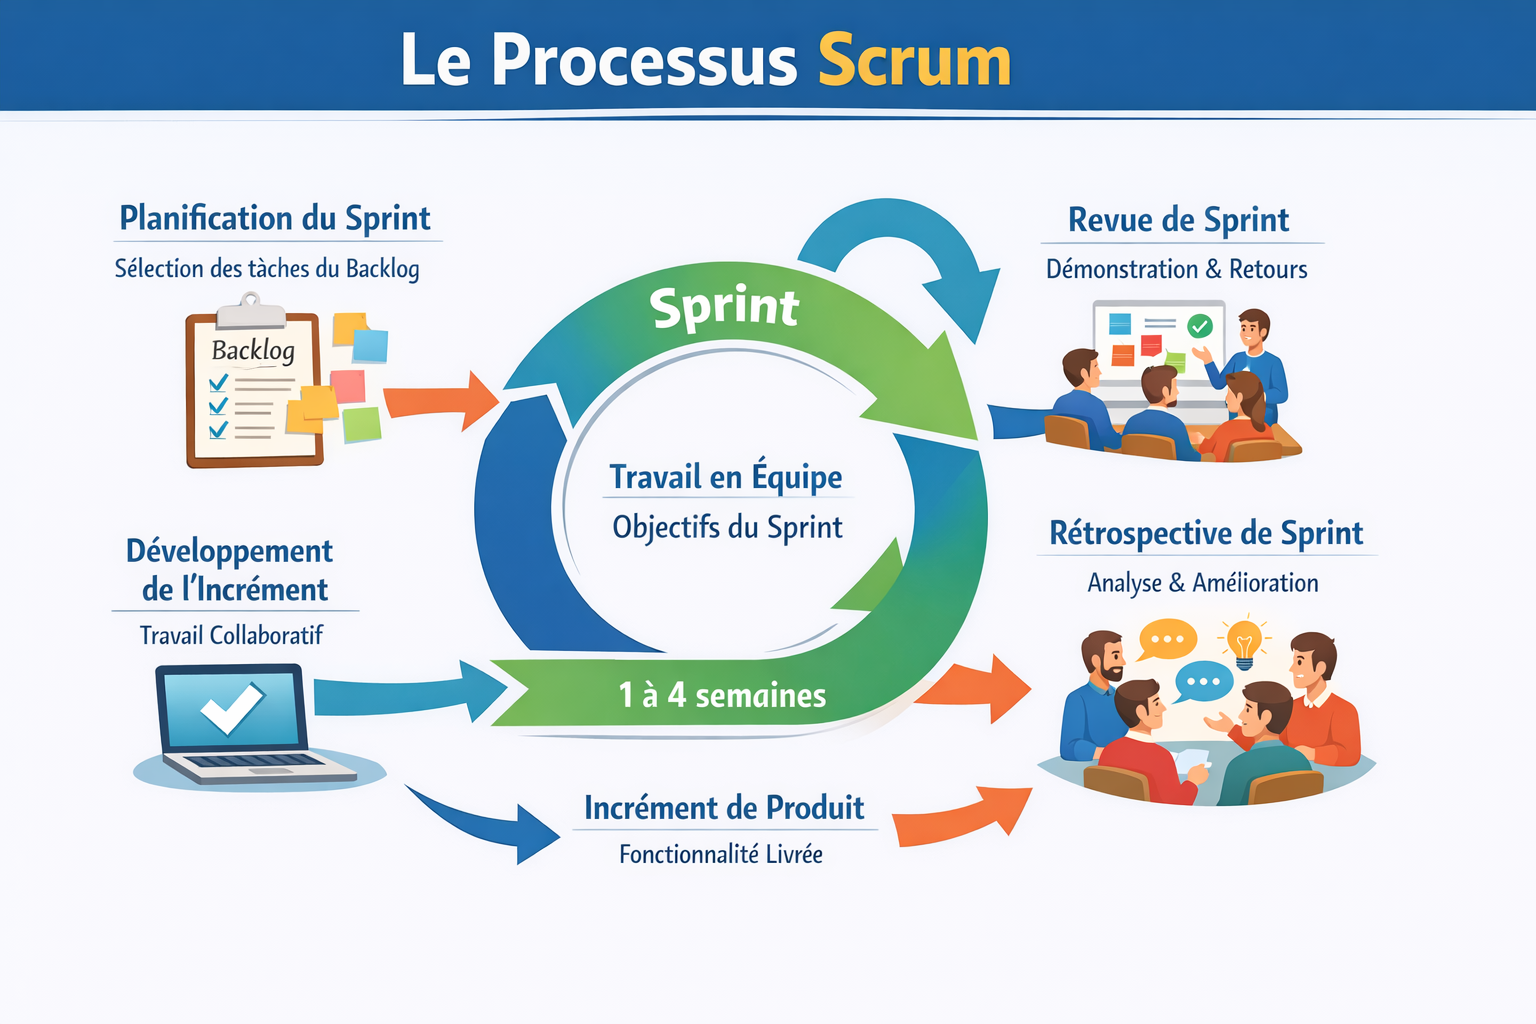
\includegraphics[width=0.7\textwidth]{scrum.png}
    \caption{Formulaire d'ajout et de modification d'un utilisateur}
    \label{fig:ui-users-form}
\end{figure}

La Figure \ref{fig:ui-users-form} illustre l'interface de gestion des profils où l'Administrateur renseigne les coordonnées et assigne les rôles. La cohérence des données est garantie par une double validation systématique 
% -----------------------------------------------------------
\subsection{Journal d'audit}
% -----------------------------------------------------------
Le module d'audit \ref{fig:ui-audit-list} assure la traçabilité complète en enregistrant automatiquement chaque action sensible. Pour chaque opération, le système archive l'identité de l'auteur, la nature de la modification (valeurs avant/après) et l'horodatage, garantissant ainsi l'intégrité et la surveillance du système.
\newpage
\begin{figure}[htbp]
    \centering
    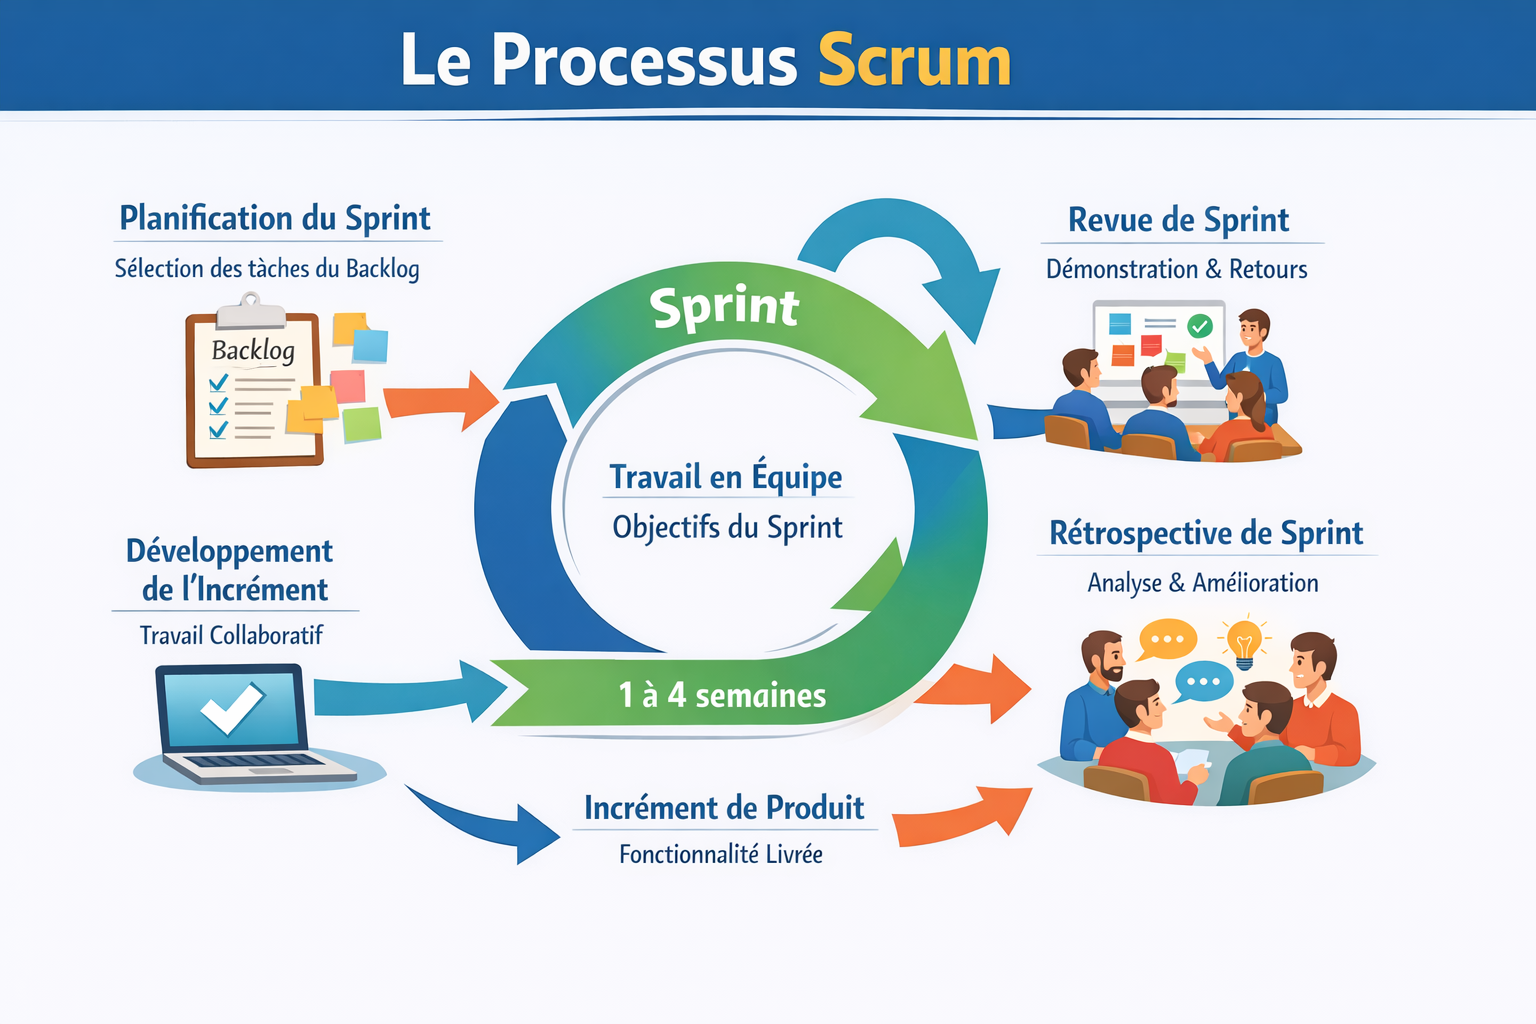
\includegraphics[width=0.70\textwidth]{scrum.png}
    \caption{Journal d'audit — Liste des actions enregistrées}
    \label{fig:ui-audit-list}
\end{figure}

La figure~\ref{fig:ui-audit-list} illustre l'interface de consultation du journal 
d'audit, accessible aux rôles Admin et RH. Les entrées peuvent être filtrées par 
date, par utilisateur et par type d'action, permettant un audit ciblé et rapide 
des événements système.

% -----------------------------------------------------------
\subsection{Gestion Organisationnelle}
% -----------------------------------------------------------
Le module de gestion organisationnelle permet aux Administrateurs 
et au RH de définir et de maintenir la structure hiérarchique de l'entreprise.

\begin{figure}[htbp]
    \centering
    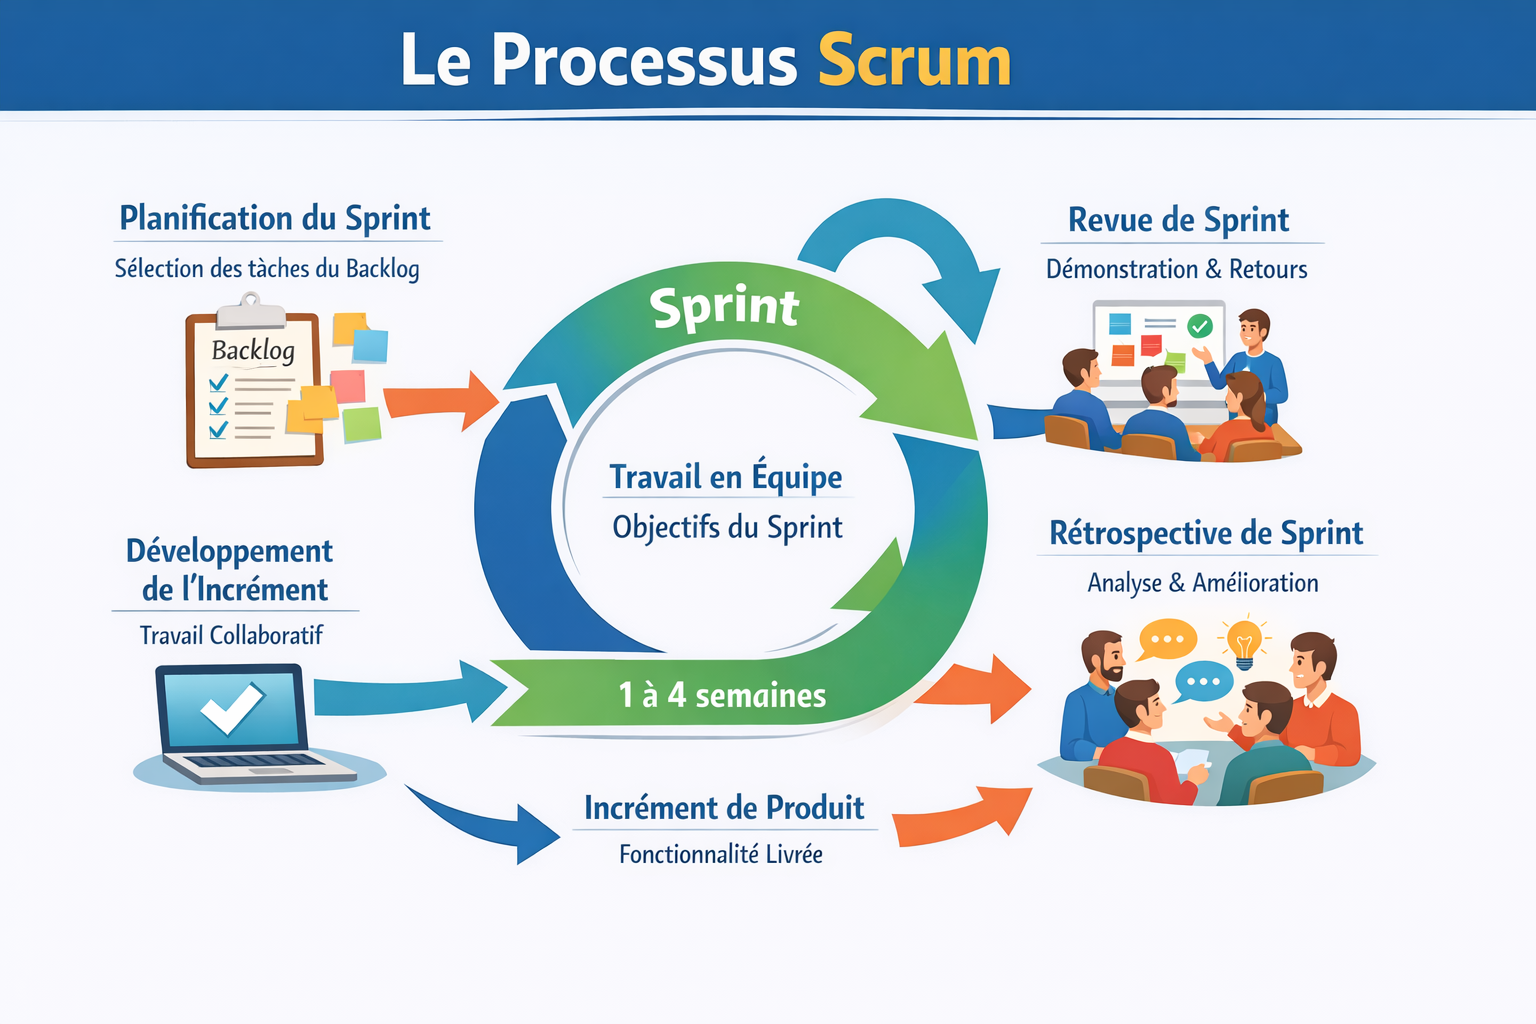
\includegraphics[width=0.70\textwidth]{scrum.png}
    \caption{Interface de gestion des départements et postes}
    \label{fig:ui-org}
\end{figure}

La Figure \ref{fig:ui-org} présente l'interface de gestion des départements et des postes. Elle permet aux administrateurs et RH de piloter la structure organisationnelle, tout en garantissant l'intégrité des données par un contrôle strict des dépendances lors de la désactivation d'un service.
% ============================================================
\section{Tests et Validation}
\label{sec:s1-tests}
% ============================================================
La phase de tests et de validation constitue une composante essentielle du cycle 
de développement agile. Elle vise à vérifier la conformité des fonctionnalités 
implémentées par rapport aux User Stories initialement définies, à identifier et 
corriger les anomalies avant la livraison au Product Owner, et à garantir la 
fiabilité, la robustesse et la qualité globale de la solution PaieZone.

% -----------------------------------------------------------
\subsection{Plan de tests}
% -----------------------------------------------------------
Afin de garantir la qualité logicielle du projet \pz, une stratégie de test 
multiniveaux a été adoptée lors du Sprint~1. Cette approche s'articule autour 
des axes suivants~:

\begin{itemize}[label=\textbullet, leftmargin=0.6cm]

    \item \textbf{Tests unitaires~:} Validation de la logique métier isolée, 
    notamment les mécanismes d'authentification JWT (génération, validation, 
    expiration du token), le Tenant Provisioning (création du schéma PostgreSQL) 
    et la génération des tokens d'invitation.

    \item \textbf{Tests d'intégration~:} Vérification de la cohérence des flux 
    entre les couches applicatives et la base de données de test~: inscription 
    multi-tenant avec isolation des schémas, persistance des journaux d'audit 
    et contrôle des accès RBAC.

    \item \textbf{Tests fonctionnels~:} Évaluation du comportement des interfaces 
    Angular~: formulaires d'inscription et de connexion, gestion des erreurs de 
    validation, redirection différenciée par rôle et filtrage du journal d'audit.
\end{itemize}

Cette approche rigoureuse garantit la fiabilité technique de la solution ainsi que sa conformité aux besoins métiers identifiés. Le Tableau \ref{tab:tests-sprint1} récapitule les principaux scénarios de test exécutés durant ce sprint pour valider ces exigences.

\renewcommand{\arraystretch}{1.3}
\begin{small}
\begin{xltabular}{\textwidth}{|c|>{\raggedright\arraybackslash}X|>{\raggedright\arraybackslash}p{4cm}|c|}
\hline
\rowcolor[gray]{0.9}
\textbf{ID} & \textbf{Description} & \textbf{Résultat attendu} & \textbf{Statut} \\
\hline
\endfirsthead
\hline
\rowcolor[gray]{0.9}
\textbf{ID} & \textbf{Description} & \textbf{Résultat attendu} & \textbf{Statut} \\
\hline
\endhead
\hline
\endfoot
\hline
\caption{Récapitulatif des cas de test du Sprint~1}
\label{tab:tests-sprint1}
\endlastfoot

T-1.1 & Authentification avec identifiants valides
& Token JWT généré, redirection vers le tableau de bord du rôle
& \textcolor{green!60!black}{\textbf{OK}} \\ \hline
T-1.2 & Authentification avec un compte désactivé ou identifiants invalides
& Accès refusé, message d'erreur générique affiché
& \textcolor{green!60!black}{\textbf{OK}} \\ \hline
T-1.3 & Authentification avec code 2FA invalide (Super Admin)
& Accès refusé, invitation à ressaisir le code TOTP
& \textcolor{green!60!black}{\textbf{OK}} \\ \hline
T-2.1 & Inscription d'une nouvelle entreprise (Tenant Provisioning)
& Schéma PostgreSQL créé, migrations Liquibase appliquées
& \textcolor{green!60!black}{\textbf{OK}} \\ \hline
T-2.2 & Inscription avec un matricule fiscal déjà enregistré
& Blocage avec message d'erreur explicite
& \textcolor{green!60!black}{\textbf{OK}} \\ \hline
T-3.1 & Création d'un utilisateur avec attribution de rôle
& Compte persisté en base avec les droits associés
& \textcolor{green!60!black}{\textbf{OK}} \\ \hline
T-3.2 & Envoi d'une invitation par e-mail et acceptation
& Token généré, e-mail envoyé, compte activé après définition du mot de passe
& \textcolor{green!60!black}{\textbf{OK}} \\ \hline
T-3.3 & Désactivation d'un utilisateur actif
& Accès révoqué immédiatement, statut mis à jour en base
& \textcolor{green!60!black}{\textbf{OK}} \\ \hline
T-4.1 & Enregistrement automatique des actions dans le journal d'audit
& Entrée créée avec (action, entité, auteur, IP, date, valeurs avant/après)
& \textcolor{green!60!black}{\textbf{OK}} \\ \hline
T-5.1 & Création d'un département et d'un poste rattaché
& Structure organisationnelle mise à jour avec succès
& \textcolor{green!60!black}{\textbf{OK}} \\ \hline
T-5.2 & Tentative de désactivation d'un département contenant des postes actifs
& Désactivation bloquée, message d'alerte affiché
& \textcolor{green!60!black}{\textbf{OK}} \\ \hline
\end{xltabular}
\end{small}
\renewcommand{\arraystretch}{1.0}

% -----------------------------------------------------------
\subsection{Tests automatisés}
% -----------------------------------------------------------

Afin de renforcer la fiabilité du Sprint~1, des tests automatisés ont été
mis en place pour valider les deux composantes les plus critiques de cette
itération~: l'isolation multi-tenant et la sécurité des accès.

\paragraph{Tests unitaires --- TenantContextService (JUnit~5 + Mockito)}
Le service \texttt{TenantContextService} est le gardien de l'architecture
multi-tenant de \pz{}~: il résout le \texttt{companyId} de chaque utilisateur
connecté et filtre toutes les requêtes JPA en conséquence. Quatorze cas de test
ont été écrits et exécutés~:

\begin{itemize}[label=\textbullet, leftmargin=0.6cm, itemsep=2pt]
    \item \textbf{Super Admin~:} \texttt{getCurrentCompanyId()} retourne \texttt{null}
    (accès global, aucun filtre appliqué sur les données).
    \item \textbf{Admin avec profil~:} le \texttt{companyId} est correctement résolu
    depuis son \texttt{UserProfile} en base.
    \item \textbf{Fallback~:} sans \texttt{UserProfile}, résolution via le champ
    \texttt{adminLogin} de la table \texttt{Company}.
    \item \textbf{Fail-closed~:} un utilisateur sans entreprise résolue reçoit
    \texttt{companyId = -1L}, bloquant tout accès aux données --- aucune fuite
    par défaut.
    \item \textbf{Accès croisé~:} \texttt{canAccessCompany(autreId)} retourne
    \texttt{false} pour toute entreprise n'appartenant pas à l'utilisateur.
\end{itemize}

\textbf{Résultat~:} 14/14 tests passés (\textcolor{green!60!black}{\textbf{OK}}).

\paragraph{Tests End-to-End --- Cypress}
Des scénarios Cypress ont automatisé la vérification de la couche sécurité~:
connexion avec identifiants valides (redirection vers le tableau de bord du rôle),
connexion échouée (maintien sur la page login), accès direct à \texttt{/paiezone/saas-dash}
sans authentification (redirection vers login), et vérification que les endpoints
\texttt{/api/companies} et \texttt{/api/dashboard/stats} retournent HTTP~401 sans token.

% ============================================================
\section{Rituels Agiles et Clôture du Sprint}
\label{sec:s1-rituels}
% ============================================================
La méthodologie Scrum impose, à la fin de chaque sprint, la tenue de deux rituels 
essentiels~: la Sprint Review et la Sprint Retrospective. Ces cérémonies garantissent 
la transparence et l'amélioration continue au sein de l'équipe PaieZone, en 
permettant respectivement d'inspecter le travail accompli et d'adapter les pratiques 
pour le sprint suivant.

% -----------------------------------------------------------
\subsection{Revue du Sprint (Sprint Review)}
% -----------------------------------------------------------

La Sprint Review a réuni l'équipe de développement, le Product Owner et les parties
prenantes. Les démonstrations ont couvert le flux d'authentification avec provisionnement
multi-tenant, la gestion des départements et postes, le journal d'audit ainsi que
l'interface Super Admin de gestion des abonnements SaaS. L'ensemble des 19 User Stories
planifiées a été validé par le Product Owner, confirmant la conformité des livrables
aux critères d'acceptation.

% -----------------------------------------------------------
\subsection{Rétrospective du Sprint (Sprint Retrospective)}
% -----------------------------------------------------------

La rétrospective a permis à l'équipe de réfléchir sur trois axes :

\begin{itemize}
    \item \textbf{Ce qui a bien fonctionné :}
    Une bonne collaboration entre les équipes front-end et back-end, assurant
    une intégration fluide et une traçabilité complète des actions.

    \item \textbf{Problèmes rencontrés :}
    La mise en place du multi-tenant s'est révélée plus complexe que prévu,
    retardant légèrement les tests d'intégration.

    \item \textbf{Actions d'amélioration :}
    Anticiper les tâches techniques en début de sprint et renforcer
    les tests d'intégration pour détecter les anomalies plus tôt.
\end{itemize}

% ============================================================
\section*{Conclusion}
\label{sec:s1-conclusion}
\addcontentsline{toc}{section}{Conclusion}
% ============================================================
Ce chapitre a présenté la réalisation du Sprint~1 de PaieZone~RH,
qui marque l'établissement du socle technique et fonctionnel de la
  plateforme. Les dix-neuf User Stories validées (authentification
  sécurisée , Tenant Provisioning, gestion des abonnements
  SaaS, administration des utilisateurs avec flux d'invitation, journal
  d'audit automatique et structuration organisationnelle )constituent
  les fondations sur lesquelles s'appuieront tous les sprints ultérieurs.

  La cohérence entre la conception UML, les interfaces Angular livrées
  et les entités JPA garantit
  une architecture robuste et extensible. Le chapitre suivant présente
  les travaux du Sprint~2, consacré à la gestion du capital humain~:
  création et administration des dossiers employés, cycle de vie des
  contrats de travail et gestion documentaire.
